\documentclass{article}

\usepackage{biblatex}
\usepackage{listings}
\usepackage{xcolor}
\usepackage{amsthm}
\usepackage{amsmath}
\usepackage{amssymb}
\usepackage{array}
\usepackage{graphicx}
\usepackage{float}
\usepackage{enumitem}


\setlist[description]{leftmargin=\parindent,labelindent=\parindent, nosep}

\graphicspath{ {./images/} }
 
\definecolor{codegreen}{HTML}{689f38}
\definecolor{codegray}{HTML}{000000}
\definecolor{codeorange}{HTML}{e65100}
\definecolor{backcolour}{HTML}{fafafa}
\definecolor{rulecolor}{HTML}{696969}
 
\lstdefinestyle{codestyle}{
    backgroundcolor=\color{backcolour},
    commentstyle=\color{codeorange},
    keywordstyle=\color{red},
    stringstyle=\color{codegreen},
    basicstyle=\small\ttfamily,
    breaklines=true,
    breakatwhitespace=false,
    captionpos=b,
    keepspaces=true,
    numbers=none,
    showtabs=false,           
    showspaces=false,
    showstringspaces=false,
    tabsize=2,
    numbersep=10pt,
    numberstyle=\small\color{rulecolor},
    frame=leftline,
    rulecolor=\color{rulecolor}
}
 
\lstset{style=codestyle}

\theoremstyle{definition}
\newtheorem{df}{Def}
\newtheorem{ex}{Example}[subsection]

\theoremstyle{remark}
\newtheorem*{rem}{Remark}
\newtheorem*{nb}{Note}


\newcommand{\func}[2]{\noindent\lstinline{#1}\\#2}


\begin{document}

\title{ OpenCV-Python for Data Science  }
\author{Michael Komodromos}
\date{ }
\maketitle

\setcounter{tocdepth}{2}
\tableofcontents
\newpage

\section{Introduction}

OpenCV is a library that includes several hundred computer vision (CV) algorithms. It was started in 1999 by Gary Bradsky and first released in 2000. OpenCV supports a wide range of programming languages such as: C++, Java, JavaScript and Python.

\subsection{OpenCV-Python}

OpenCV-Python brings together the best qualities of OpenCV and Python. Allowing for great performance and the stylistic qualities of Python. This is achieved by creating Python wrappers around the C/C++ modules. Meaning code is just as fast as if it was written in C/C++ (as C/C++ is being executed in the background).

The Python OpenCV modules are used in conjunction with numpy, a highly optimized library for numerical operations. Providing a MATLAB style syntax. In the background OpenCV array structures are converted to and from Numpy arrays.

\begin{rem}
OpenCV Python is the appropriate tool for fast prototyping.
\end{rem}

\subsection{Installation}

The following installation instructions are for Python version 3.6+. It is possible to use older version of Python, however unless there is a specific reason to do so, it is not recommended. 

\begin{rem}
Python version 3.6 comes with python-venv. The module allows you to easily create virtual environments.
\end{rem}

\begin{nb}
Virtual environments become extremely useful and future proofs your system from mismatched dependencies. 
\end{nb}

\subsubsection{Setting up a virtual environment}

From your terminal run the following: 
\begin{lstlisting}[language=bash]
python3 -m venv env
. env/bin/activate
\end{lstlisting}

You should now see \lstinline{(env)} at the start of the command line.


\subsubsection{Installing OpenCV-Python}

\begin{lstlisting}[language=bash]
pip install opencv-python
\end{lstlisting}


That's it! All dependencies (numpy) are installed alongside opencv. To test everything is working type:
\begin{lstlisting}[language=Python]
>>> import cv2
\end{lstlisting}




\break





\section{Numpy}

Basic knowledge of nunpy is needed to work with OpenCV. Working knowledge of Python is assumed.

\subsection{Arrays}

The main object in Numpy is the homogeneous multidimensional array. A table of elements typically numbers all of the same type.

\begin{rem}
homogeneous implies that all elements are of the same type.
\end{rem}

\begin{nb}
In numpy dimensions are called axes
\end{nb}

\begin{ex} A numpy array type
\begin{lstlisting}[language=Python]
[[ 1., 0., 0.],
 [ 0., 1., 2.]]
\end{lstlisting}
2 axes, length 3
\end{ex}

Numpy's array class is called \lstinline{ndarray}. It is also know by \lstinline{array} in the numpy namespace of course.


\subsubsection{Creating Arrays}

There are several ways to create arrays. \textit{Note:} the array type is deduced from the type of the elements in the sequence. 

\begin{ex} Creating arrays in numpy
\begin{lstlisting}[language=Python]
>>> import numpy as np
>>> a = np.array([1, 2, 3])
\end{lstlisting}
Creates a 1 dimensional, or an array with 1 axis, of type int64.
\end{ex}

The \lstinline{array} function transforms multiple sequences into the respective multidimensional array.

\begin{ex} Creating a 3 dimensional array
\begin{lstlisting}[language=Python]
>>> b = np.array([
    [
        [1,2,3],
        [2,3,4]
    ],
    [
        [3,4,5],
        [4,5,6]
    ]
])
>>> b.ndim
3
\end{lstlisting}
\end{ex}

\begin{nb}
    The data type can be set with the dtype parameter\\ \textit{ex:} \lstinline{np.array( [ [1,2], [3,4] ], dtype=complex)}
\end{nb}


\subsubsection{Attributes}

\noindent\textbf{ndim}\\
returns number of axes.\\

\noindent\textbf{shape}\\
returns a tuple with the number of rows \lstinline{n} and the number of columns \lstinline{m} \textit{i.e.} \lstinline{(n, m)}.\\

\noindent\textbf{size}\\
returns total number of elements in array.\\

\noindent\textbf{dtype}\\
returns an object describing the elements data type, float64, int64 etc.

\subsubsection{Functions}


\func{np.zeros(shape, dtype=float, order='C')}{Creates an array full of zeros.}

\begin{ex} np.zeros
\begin{lstlisting}[language=Python]
>>> np.zeros((5, 7))
\end{lstlisting}
\end{ex}


\func{np.ones(shape, dtype=float, order='C')}{Creates an array full of ones.}

\begin{ex} np.ones
\begin{lstlisting}[language=Python]
>>> np.ones((1, 3))
\end{lstlisting}
\end{ex}

\func{np.empty(shape, dtype=float, order='C')}{Creates an array whose initial content is random.}

\begin{ex} np.empty
\begin{lstlisting}[language=Python]
>>> np.empty((3,4))
\end{lstlisting}
\end{ex}

\func{np.full(shape, val, dtype=None, order='C')}{Return a new array of given shape and type, filled with val.}

\begin{ex} np.full
\begin{lstlisting}[language=Python]
>>> np.full((3,4), 42)
\end{lstlisting}
\end{ex}


\func{np.arange(start, stop, step, dtype=None)}{similar to native \lstinline{range} function, but returns anumpy array object.}

\begin{ex} np.arange
\begin{lstlisting}[language=Python]
>>> np.arange(0, 100, 5)
\end{lstlisting}
\end{ex}

\func{np.linspace(start, stop, num=50, endpoint=True, retstep=False, dtype=None, axis=0)}{returns an array of floating point integers, that are linearly spaced.}

\begin{ex} np.linespace
\begin{lstlisting}[language=Python]
>>> np.linspace(0,2,9)
\end{lstlisting}
\end{ex}


\break

\subsection{Basic Operations}

Arithmetic operations on arrays are applied elementwise, resulting in an new array being created and filled with the result.

\begin{ex} Arithmetic
\begin{lstlisting}[language=Python]
>>> a = np.ones(3)
>>> b = np.zeros(3)
>>> b[1] = 5
>>> a * 5
array([ 5., 5., 5.]
>>> a * b
array([0., 5., 0.])
\end{lstlisting}
\end{ex}

\begin{nb}
    the matrix product can be performed using the \lstinline{@} operator, or with the \lstinline{dot()} method.
\end{nb}

\begin{ex} Matrix Multiplication
\begin{lstlisting}[language=Python]
>>> A = np.array([[1,2],[0,1]])
>>> B = np.array([[2,0],[3,4]])
>>> A @ B
array([[5, 4],
       [3, 4]])
>>> A.dot(B)
array([[5, 4],
       [3, 4]])
\end{lstlisting}
\end{ex}

\noindent
Some operators like \lstinline{+=} and \lstinline{*=} modify the existing array.

\begin{ex} Modifying arrays
\begin{lstlisting}[language=Python]
>>> a = np.ones((2,3), dtype=int)
>>> b = np.random.random((2,3))
>>> a *= 3
>>> a
array([[3, 3, 3],
       [3, 3, 3]])
>>> b += a
>>> b
array([[ 3.417022  ,  3.72032449,  3.00011437],
       [ 3.30233257,  3.14675589,  3.09233859]])
\end{lstlisting}
\end{ex}

\subsubsection{Unary Operation}

\begin{df}Unary Operations

An operation that takes a single operand. \textit{ex:} \lstinline{not} is an operation that logically negates an expression.  
\end{df}

\func{np.sum(axis=None, dtype=None, out=None,  where=True)}{Returns the sum of all elements in an array}

\begin{ex} np.sum
\begin{lstlisting}[language=Python]
>>> a = np.ones(2)
>>> a.sum()
2
\end{lstlisting}
\end{ex}

\func{np.min(iterable, *args)}{Returns the minimum element of an array.}

\begin{ex} np.min
\begin{lstlisting}[language=Python]
>>> a = np.array([1, 5, 10])
>>> a.min()
1
\end{lstlisting}
\end{ex}

\func{np.max(iterable, *args)}{Returns the maximum element of an array.}

\begin{ex} np.max
\begin{lstlisting}[language=Python]
>>> a = np.array([1, 5, 10])
>>> a.max()
10
\end{lstlisting}
\end{ex}


\subsubsection{Universal Functions}

Numpy provides many familiar mathematical functios.\\

\func{np.sin(x, out=None, *args)}{Applies the sine operation on a given data type.}

\begin{ex} np.sin
\begin{lstlisting}[language=Python]
>>> A = np.arange(3)
>>> np.sin(B)
array([0.        , 0.84147098, 0.90929743])
\end{lstlisting}
\end{ex}

\func{np.exp(x, out=None, *args)}{Applies an exponential operation to a given data type.}

\begin{ex} np.exp
\begin{lstlisting}[language=Python]
>>> A = np.arange(3)
>>> np.exp(A)
array([ 1.        ,  2.71828183,  7.3890561 ])
\end{lstlisting}
\end{ex}

\func{np.cumsum(a, axis=None, dtype=None, out=None)}{Returns an array comataining the cumulative sum of elements.}

\begin{ex} np.cumsum
\begin{lstlisting}[language=Python]
>>> A = np.ones(3)
>>> np.cumsum(A)
array([ 1.,  2., 3.])
\end{lstlisting}
\end{ex}

\begin{table}[h!]
    \centering
    \begin{tabular}{p{2cm} p{10cm}}
    \hline
    Function & Operation \\
    \hline
    \textbf{all} & whether elements along an axis evaluate to a truthy value \\
    \textbf{any} & Tests whether any element along an axis evaluates to a truthy value \\
    \textbf{argmax} & returns the indecie of the maximum values along and axis \\
    \textbf{argmin} & returns the indicie of the miimum values along and axis \\
    \textbf{average} & computes the weighted average along a given axis \\
    \textbf{bincount} & counts the number of occurrences of each value in an array of non negative integers \\
    \textbf{ceil} & returns the ceiling of an array element wise; \textit{i.e.} the smallest int \textit{i} such that $ i \ge x$ \\
    \textbf{clip} & given an interval $ a \le i \le b $ element $ i $ outside the interval is set to the interval edges \\
    \textbf{conj} & returns the complex conjugate element wise \\
    \textbf{corrcoef} & returns the Pearson product moment correlation coefficient \\
    \textbf{cov} & estimates a covariance matrix given data and weights \\
    \textbf{cross} & returns the cross product of two vectors \\
    \textbf{cumprod} & returns the cumulative product of elements along a given axis \\
    \textbf{cumsum} & return the cumulative sum of elements along a given axis \\
    \textbf{diff} & calculate the n-th discrete difference along the given axis \\
    \textbf{dot} & dot product of two arrays \\
    \textbf{floor} & return the floor of the input, element-wise \\
    \textbf{inner} & inner product of two arrays \\
    \textbf{maximum} & element-wise maximum of array elements \\
    \textbf{mean} & compute the arithmetic mean along the specified axis \\
    \textbf{median} & compute the median along the specified axis \\
    \textbf{minimum} & element-wise minimum of array elements \\
    \textbf{nonzero} & return the indices of the elements that are non-zero \\
    \textbf{outer} & compute the outer product of two vectors \\
    \textbf{prod} & return the product of array elements over a given axis \\
    \textbf{sort} & return a sorted copy of an array \\
    \textbf{std} & compute the standard deviation along the specified axis \\
    \textbf{sum} & sum of array elements over a given axis \\
    \textbf{trace} & return the sum along diagonals of the array \\
    \textbf{transpose} & permute the dimensions of an array \\
    \textbf{var} & compute the variance along the specified axis. \\
    \textbf{vdot} & return the dot product of two vectors \\
    \textbf{where} & return elements chosen from x or y depending on condition \\
    \hline
\end{tabular}
\caption{functions in numpy}
\label{table:1}
\end{table}

\clearpage
    
\subsubsection{Indexing, Slicing and Iterating}

One-dimensional arrays can be indexed, sliced and iterated over, similar to native python lists.

\begin{ex}Indexing 
\begin{lstlisting}[language=Python]
>>> a = np.arange(10)**3
>>> a
array([  0,   1,   8,  27,  64, 125, 216, 343, 512, 729])
>>> a[2]
8
\end{lstlisting}
\end{ex}

\begin{ex}Slicing
\begin{lstlisting}[language=Python]
>>> a[2:5]
array([ 8, 27, 64])
\end{lstlisting}
\end{ex}

\begin{ex}Iterating
\begin{lstlisting}[language=Python]
>>> a[:6:2] = -1000    # equivalent to a[0:6:2] = -1000; from start to position 6, exclusive, set every 2nd element to -1000
>>> a
array([-1000,     1, -1000,    27, -1000,   125,   216,   343,   512,   729])
>>> a[ : :-1] # reversed
array([  729,   512,   343,   216,   125, -1000,    27, -1000,     1, -1000])
>>> for i in a:
...     print(i)
...
0
1
\end{lstlisting}
\end{ex}

\noindent Multidimensional arrays can have one index per axis.

\begin{ex}Indexing Multidimensional Arrays
\begin{lstlisting}[language=Python]
>>> def f(x,y):
...     return 10*x+y
...
>>> b = np.fromfunction(f,(5,4),dtype=int)
>>> b
array([[ 0,  1,  2,  3],
       [10, 11, 12, 13],
       [20, 21, 22, 23],
       [30, 31, 32, 33],
       [40, 41, 42, 43]])
>>> b[2,3]
23
\end{lstlisting}
\end{ex}

\begin{ex}Slicing Multidimensional Arrays
\begin{lstlisting}[language=Python]
>>> b[0:5, 1] # each row in the second column of b
array([ 1, 11, 21, 31, 41])
>>> b[ : ,1]  # equivalent to the previous example
array([ 1, 11, 21, 31, 41])
>>> b[1:3, : ] # columns in the second and third row of b
array([[10, 11, 12, 13],
       [20, 21, 22, 23]])
\end{lstlisting}
\end{ex}

\begin{ex} Iterating over Multidimensional Arrays
\begin{lstlisting}[language=Python]
>>> for row in b:
...     print(row)
...
[0 1 2 3]
[10 11 12 13]
[20 21 22 23]
[30 31 32 33]
[40 41 42 43]
\end{lstlisting}
\end{ex}

\begin{nb}
    Iterating is done w.r.t. the first axis
\end{nb}

The \lstinline{flat} attribute can be used to create an iterator over all the elements in an array

\begin{ex}The \lstinline{flat} attribute
\begin{lstlisting}[language=Python]
>>> for element in b.flat:
...     print(element)
...
0
1
2
# truncated
\end{lstlisting}
\end{ex}


\break


\subsection{Shape Manipulation}

\subsubsection{Changing the shape of an array}

An array's shape is determined by the number of elements along each axis.

\begin{ex}Array shape
\begin{lstlisting}[language=Python]
>>> a = np.floor(10*np.random.random((3,4)))
>>> a.shape
(3, 4)
\end{lstlisting}
\end{ex}

\noindent Various methods are used to change the shape of an array.\\


\func{np.ravel(a, order='C')}{Returns a flatten version of an array.}

\begin{ex} np.ravel
\begin{lstlisting}[language=Python]
>>> a.ravel()
array([ 2.,  8.,  0.,  6.,  4.,  5.,  1.,  1.,  8.,  9.,  3.,  6.])
\end{lstlisting}
\end{ex}


\begin{nb}
    The command produces the same output as \lstinline{np.array(list(a.flat))}\\
\end{nb}


\func{np.reshape(a, newshape, order='C')}{Returns an array with a modified shape.}

\begin{ex} np.reshape
\begin{lstlisting}[language=Python]
>>> a.reshape(6,2)
array([[ 2.,  8.],
       [ 0.,  6.],
       ...
       [ 3.,  6.]])
\end{lstlisting}
\end{ex}

\begin{nb}
If a dimension of $ -1 $ is given then the dimension is automatically calculated.\\
\end{nb}


\func{ndarray.T}{Returns the transposed array.}

\begin{ex} T
\begin{lstlisting}[language=Python]
>>> a.T  # returns the array, transposed
array([[ 2.,  4.,  8.],
       [ 8.,  5.,  9.],
       [ 0.,  1.,  3.],
       [ 6.,  1.,  6.]])
\end{lstlisting}
\end{ex}

\begin{nb}
The \lstinline{resize} method modifies the array itself.
\end{nb}

\subsubsection{Stacking arrays}

Several arrays can be stacked together along different axes.\\

\func{np.vstack(tup)}{Stacks arrays in sequence vertically (row wise).}

\begin{ex} np.vstack
\begin{lstlisting}[language=Python]
>>> a = np.floor(10*np.random.random((2,2)))
>>> a
array([[ 8.,  8.],
       [ 0.,  0.]])
>>> b = np.floor(10*np.random.random((2,2)))
>>> b
array([[ 1.,  8.],
       [ 0.,  4.]])
>>> np.vstack((a,b))
array([[ 8.,  8.],
       [ 0.,  0.],
       [ 1.,  8.],
       [ 0.,  4.]])
\end{lstlisting}
\end{ex}


\func{np.hstack(tup)}{Stacks arrays in sequence horizontally (col wise).}

\begin{ex} np.hstack
\begin{lstlisting}[language=Python]
>>> np.hstack((a,b))
array([[ 8.,  8.,  1.,  8.],
       [ 0.,  0.,  0.,  4.]])
\end{lstlisting}
\end{ex}

\func{np.column_stack(tup)}{Stack 1D arrays as columns into 2D arrays.}

\begin{ex} np.column\_stack
\begin{lstlisting}[language=Python]
>>> a = np.array((1,2,3))
>>> b = np.array((2,3,4))
>>> np.column_stack((a,b))
array([[1, 2],
       [2, 3],
       [3, 4]])
\end{lstlisting}
\end{ex}

\func{np.concatenate((a1, a2, ...), axis=0, out=None)}{Join a sequence of arrays along an existing axis.}

\begin{ex} np.concatenate
\begin{lstlisting}[language=Python]
>>> a = np.array([[1, 2], [3, 4]])
>>> b = np.array([[5, 6]])
>>> np.concatenate((a, b), axis=0)
array([[1, 2],
       [3, 4],
       [5, 6]])
>>> np.concatenate((a, b.T), axis=1)
array([[1, 2, 5],
       [3, 4, 6]])
>>> np.concatenate((a, b), axis=None)
array([1, 2, 3, 4, 5, 6])
\end{lstlisting}
\end{ex}

\subsubsection{Splitting Arrays}

\func{np.hsplit(arr, indices_or_sections)}{Splits an array along its horizontal axis.}

\begin{ex} np.hsplit
\begin{lstlisting}[language=Python]
>>> x = np.arange(16.0).reshape(4, 4)
>>> x
array([[ 0.,   1.,   2.,   3.],
       [ 4.,   5.,   6.,   7.],
       [ 8.,   9.,  10.,  11.],
       [12.,  13.,  14.,  15.]])
>>> np.hsplit(x, 2)
[array([[  0.,   1.],
       [  4.,   5.],
       [  8.,   9.],
       [12.,  13.]]),
 array([[  2.,   3.],
       [  6.,   7.],
       [10.,  11.],
       [14.,  15.]])]
\end{lstlisting}
\end{ex}


\func{np.vsplit(arr, indices_or_sections)}{Splits an array along the vertical axis (row wise).}

\begin{ex}\lstinline{}
\begin{lstlisting}[language=Python]
>>> np.vsplit(x, 2)
[array([[0., 1., 2., 3.],
       [4., 5., 6., 7.]]), array([[ 8.,  9., 10., 11.],
       [12., 13., 14., 15.]])]
\end{lstlisting}
\end{ex}


\break


\subsection{Copies and Views}

Important to distinguish when the data of an array has been copied or not. There are three cases to consider.

\subsubsection{No Copy}

Assignments make no copy of an array. 

\begin{ex} Assignment and copying
\begin{lstlisting}[language=Python]
>>> a = np.arange(12)
>>> b = a            # no new object is created
>>> b is a           # a and b are two names for the same ndarray object
True
>>> b.shape = 3,4    # changes the shape of a
>>> a.shape
(3, 4)
\end{lstlisting}
\end{ex}


\subsubsection{Shallow Copies}

\func{ndarray.view(dtype=None, type=None)}{New view of array with the same data}

\begin{ex} ndarray.view
\begin{lstlisting}[language=Python]
>>> c = a.view()
>>> c is a
False
>>> c.base is a                        # c is a view of the data owned by a
True
>>> c.flags.owndata
False
\end{lstlisting}
\begin{nb}
The data type can be changed with the 
\end{nb}

\begin{nb}
Changes in $ c $'s data also result in $ a $'s data changing
\end{nb}
\end{ex}

\begin{rem}
Slicing arrays also result in a view being returned.
\end{rem}

\subsubsection{Deep Copies}

\func{ndarray.copy(a, order='K')}{Returns an array copy of the given object.}

\begin{ex} ndarray.copy
\begin{lstlisting}[language=Python]
>>> d = a.copy()                          # a new array object with new data is created
>>> d is a
False
\end{lstlisting}
\end{ex}


\break


\subsection{Broadcasting}

\begin{df}Broadcasting

Describes how numpy treats arrays with different shapes during arithmetic operations. The smaller array is ``broadcast'' across the larger array $ s.t. $ they have compatible shapes.
\end{df}

\begin{rem}
Numpy operations are usually done on pairs of arrays element-wise. The simplest case is that two arrays have the same shape.
\end{rem}


\begin{ex}Broadcasting simplest case
\begin{lstlisting}[language=Python]
>>> a = np.array([1.0, 2.0, 3.0])
>>> b = np.array([2.0, 2.0, 2.0])
>>> a * b
array([ 2.,  4.,  6.])
\end{lstlisting}
\end{ex}


\begin{rem}
This constraint is relaxed when an array and a scalar are combined in an operation
\end{rem}

\begin{ex}Broadcasting: arrays and scalars
\begin{lstlisting}[language=Python]
>>> a = np.array([1.0, 2.0, 3.0])
>>> b = 2.0
>>> a * b
array([ 2.,  4.,  6.])
\end{lstlisting}
\end{ex}

\noindent These rules generalize as follows, two dimensions are compatible when:

\begin{enumerate}
    \item they are equal

    \item one dimension if of length 1
\end{enumerate}

\begin{nb}
If these conditions are not met then a \lstinline{ValueError} is raised
\end{nb}

\begin{ex}Broadcasting
\begin{lstlisting}[language=Python]
A      (4d array):  8 x 1 x 6 x 1
B      (3d array):      7 x 1 x 5
Result (4d array):  8 x 7 x 6 x 5

A      (3d array):  15 x 3 x 5
B      (3d array):  15 x 1 x 5
Result (3d array):  15 x 3 x 5

A      (3d array):  15 x 3 x 5
B      (2d array):       3 x 5
Result (3d array):  15 x 3 x 5

A      (3d array):  15 x 3 x 5
B      (2d array):       3 x 1
Result (3d array):  15 x 3 x 5
\end{lstlisting}
\end{ex}


\break


\subsection{Indexing}

\subsubsection{Indexing with arrays of indices}

Arrays containing indices can be used to interact with other arrays.

\begin{ex}Indexing with arrays containing indices
\begin{lstlisting}[language=Python]
>>> a = np.arange(12) ** 2 # square numbers
>>> i = np.array([1, 1, 3, 8, 5 ]) # indices
>>> a[i] # elements at positions i
array([ 1,  1,  9, 64, 25])
\end{lstlisting}
\end{ex}

\begin{rem}
For multidimensional arrays a single array of indices refers to the first dimension
\end{rem}

\begin{nb}
Multiple indexes can be given to interact with more dimensions.
\end{nb}


\begin{ex}Indexing multidimensional arrays
\begin{lstlisting}[language=Python]
>>> a = np.arange(12).reshape(3,4)
>>> a
array([[ 0,  1,  2,  3],
       [ 4,  5,  6,  7],
       [ 8,  9, 10, 11]])
>>> i = np.array( [ [0,1], [1,2] ] )
>>> j = np.array( [ [2,1], [3,3] ] )
>>> a[i,j] # i and j must have equal shape
array([[ 2,  5],
       [ 7, 11]])
\end{lstlisting}

\begin{lstlisting}[language=Python]

# i, row entries
[ [0, 1], 
  [1, 2] ] 
# j, col entries 
[ [2, 1],
  [3, 3] ] 

# applied to
[[ 0,  1,  2,  3],
 [ 4,  5,  6,  7],
 [ 8,  9, 10, 11]]

# results 
[[ a[0, 2], a[1, 1] ], 
 [ a[1, 3], a[2, 3] ]] 

i (0, 0)  j (0, 0)      i (1, 0)  j (0, 1)
i (1, 0)  j (1, 0)      i (1, 1)  j (1, 1)

\end{lstlisting}
\end{ex}

\subsubsection{Indexing with Boolean Arrays}

Boolean indexing uses an array with the same shape as the original array in order to extract elements. A boolean operation is performed on the original array, for instance $ \le $, $ > $, $ == $, $ isnan() $ and so forth to obtain a boolean indexed array.

\begin{ex}Boolean Indexing
\begin{lstlisting}[language=Python]
>>> a = np.arange(12).reshape(3,4)
>>> b = a > 4
>>> b # boolean with a's shape
array([[False, False, False, False],
       [False,  True,  True,  True],
       [ True,  True,  True,  True]])
>>> a[b] # 1D array with the selected elements
array([ 5,  6,  7,  8,  9, 10, 11])
\end{lstlisting}
\end{ex}

\begin{rem}
Can be extremely useful for value assignment
\end{rem}

\begin{ex} Assigning values
\begin{lstlisting}[language=Python]
>>> a[b] = 0 # All elements of 'a' higher than 4 become 0
>>> a
array([[0, 1, 2, 3],
       [4, 0, 0, 0],
       [0, 0, 0, 0]])
\end{lstlisting}
\end{ex}

\begin{nb}
Alternatively a 1D boolean array can be used to extract the relevant slices of an array
\end{nb}

\begin{ex}Slicing with boolean arrays
\begin{lstlisting}[language=Python]
>>> a = np.arange(12).reshape(3,4)
>>> b1 = np.array([False,True,True]) # first dim selection
array([[ 4,  5,  6,  7],
       [ 8,  9, 10, 11]])
\end{lstlisting}
\end{ex}

\begin{nb}
The length of the array must coincide with the length of the dimension
\end{nb}


\break


\subsection{Constants}

\begin{table}[h!]
    \def\arraystretch{1.1}%
    \centering
    \begin{tabular}{p{4cm} p{2cm} p{6cm}}
	Constant & Numpy Var & Definition \\
	\hline
	Positive Infinity & \footnotesize{\textbf{PINF}} & floating point representation of positive infinity \\ 
	Negative Infinity & \footnotesize{\textbf{NINF}} & floating point representation of negative infinity \\
	Positive Zero & \footnotesize{\textbf{PZERO}} & floating point representation of positive zero \\
	Negative Zero & \footnotesize{\textbf{NZERO}} & floating point representation of negative zero \\ 
	Euler's Constant & \footnotesize{\textbf{e}} & base of natural logarithms, e = 2.718281... \\
	Pi & \footnotesize{\textbf{pi}} & pi = 3.14159... \\
	NaN & \footnotesize{\textbf{nan}} & not a number \\
    	\hline
    \end{tabular}
\caption{constants in numpy}
\label{table:2}
\end{table}




\break




\section{Matplotlib}

Matplotlib is a Python 2D plotting library used for producing publication quality figures. 

Throughout OpenCV matplotlib is used to interact with images; a basic understanding of matplotlib is required.

To install matplotlib in a given virtual environment run

\begin{lstlisting}[language=bash]
pip install matplotlib
\end{lstlisting}

\subsection{General Concepts}

Matplotlib is organised in a hierarchical structure. At the top of the hierarchy is the state-machine environment, provided by the \lstinline{matplotlib.pyplot} module. The next level down is the object-oriented interface, where the user explicitly creates and keeps track of figures and axes objects. Beyond that a purely object oriented approach can be taken for fine grain control, \textit{ie.} building GUI apps. 

\begin{df}State Machine

    A state machine consists of a set of states $ s $ and a set of events $ \Sigma $ which change the current state. In terms of matplotlib the state is a plot, typically references as \lstinline{plt} and the set of events are methods that change the plot; adding points, lines, titles etc.
\end{df}

\newpage

\subsection{The Structure of Figures}

\subsubsection{Figures}

Figure are used to keep track of the canvas, child axes, titles, legends etc. 

\begin{nb}
The canvas is responsible for drawing the plot
\end{nb}

\begin{nb}
    A figure needs at least one set of axes
\end{nb}

\begin{figure}[h!]
    \centering
    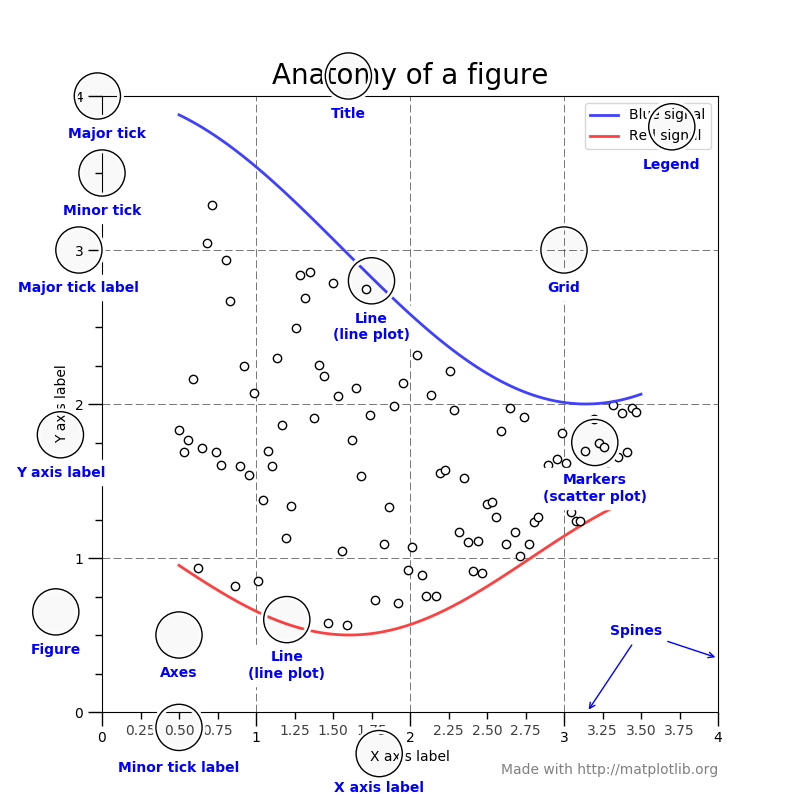
\includegraphics[width=\textwidth]{matplotlib_figure_anatomy}
    \caption{Anatomy of a matplotlib figure}
    \label{fig:mesh1}
\end{figure}

\clearpage

\subsubsection{Axes}

Axes can be thought of as a plot. A given figure can have multiple axes but an axes can only be in one figure. Axes are made up of \lstinline{Axis} objects, representing the dimensionality of the plot, \textit{i.e.} 3 axis $ \Rightarrow $ 3D plot.


\subsubsection{Axis}

Number-line like objects. The set the graph limits and generate ticks (marks along the axis) and tick labels. 


\subsubsection{Artist}

Everything that is visible on a figure is an artist: text,  Line2D , collection, patch objects and so on. All artists are drawn to the canvas.


\subsubsection{Input types}

All the plotting functions expect a numpy array as input.

\begin{nb}
Array like class like pandas data objects and numpy martix may not work as intended. It is best to convert these to numpy array object beforehand.
\end{nb}


\break


\subsection{Pyplot}

\lstinline{matplotlib.pyplot} is a collection of command style functions used to make changes to figures. Function calls states are preserved across states. 

\begin{ex}A Simple Plot
\begin{lstlisting}[language=Python]
>>> import matplotlib.pyplot as plt
>>> plt.plot([1, 2, 3, 4])
>>> plt.show()
\end{lstlisting}
\begin{figure}[h!]
    \centering
    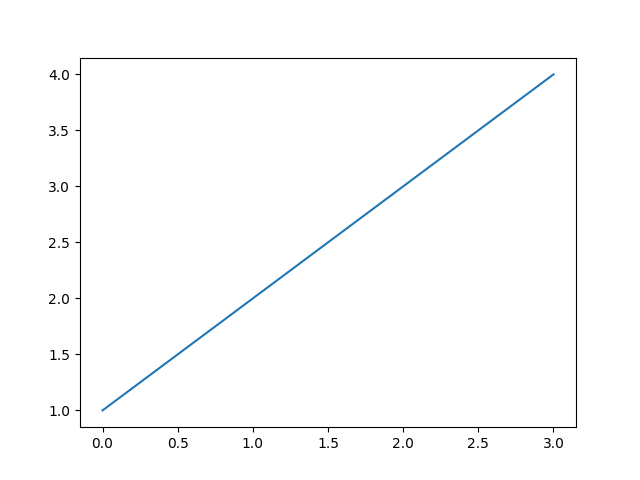
\includegraphics[width=0.5\textwidth]{matplotlib_simple_plot}
    \caption{A simple plot}
    \label{fig:simple_plot}
\end{figure}
\end{ex}

\func{pyplot.plot(*args, scalex=True, scaley=True, data=None, **kwargs)}{Plots y versus x as lines and/or markers.}

\begin{ex}pyplot.plot() command
\begin{lstlisting}[language=Python]
>>> plot(x, y) # plot x and y using default line style and color
>>> plot(x, y, 'bo') # plot x and y using blue circle markers
>>> plot(y)
>>> plot('xlabel', 'ylabel', data=obj) # plot labelled data
\end{lstlisting}
\end{ex}


\subsubsection{plot() formatting}

There are a number of formatting options available, format strings or the \lstinline{fmt} arg takes the following form: \lstinline{[marker][line][color]}. 

\begin{nb}
Other combinations are supported but their interpretation is ambiguous.
\end{nb}

\begin{table}[h!]
\centering
\begin{tabular}{ >{\centering}p{3cm} p{6cm}}
    \hline
    Character & Description \\
    \hline
    . 	& point marker \\
    , 	& pixel marker \\
    o 	& circle marker \\
    v 	& triangle\_down marker \\
    \^{}  & triangle\_up marker \\
    $ < $ & triangle\_left marker \\
    $ > $ & triangle\_right marker \\
    1 	& tri\_down marker \\
    2 	& tri\_up marker \\
    3 	& tri\_left marker \\
    4 	& tri\_right marker \\
    s 	& square marker \\
    p 	& pentagon marker \\
    $ * $ & star marker \\
    h 	& hexagon1 marker \\
    H 	& hexagon2 marker \\
    + 	& plus marker \\
    x 	& x marker \\
    D 	& diamond marker \\
    d 	& thin\_diamond marker \\
    $ \vert $ & vline marker \\
    \_ 	& hline marker \\
    \hline
\end{tabular}
\caption{Markers}
\label{table:markers}
\end{table}

\begin{table}[h!]
\centering
\begin{tabular}{ >{\centering}p{3cm} p{6cm}}
    \hline
    Character & Description \\
    \hline
    - 	& solid line style \\
    -- 	& dashed line style \\
    -. 	& dash-dot line style \\
    : 	& dotted line style \\
    \hline
\end{tabular}
\caption{Line Styles}
\label{table:line_styles}
\end{table}

\begin{table}[h!]
\centering
\begin{tabular}{ >{\centering}p{3cm} p{6cm}}
    \hline
    Character & Description \\
    \hline
    b 	& blue \\
    g 	& green \\
    r 	& red \\
    c 	& cyan \\
    m 	& magenta \\
    y 	& yellow \\
    k 	& black \\
    w 	& white \\
    \hline
\end{tabular}
\caption{Colors}
\label{table:colors}
\end{table}

\pagebreak

\begin{ex} Plot format strings
\begin{lstlisting}[language=Python]
'b'    # blue markers with default shape
'or'   # red circles
'-g'   # green solid line
'--'   # dashed line with default color
\end{lstlisting}
\end{ex}


\begin{ex} Plot formatting in practise
\begin{lstlisting}[language=Python]
>>> plt.plot([1, 2, 3, 4], [1, 4, 9, 16], '.--m')
>>> plt.axis([0, 6, 0, 20])
>>> plt.show()
\end{lstlisting}

\begin{figure}[h!]
    \centering
    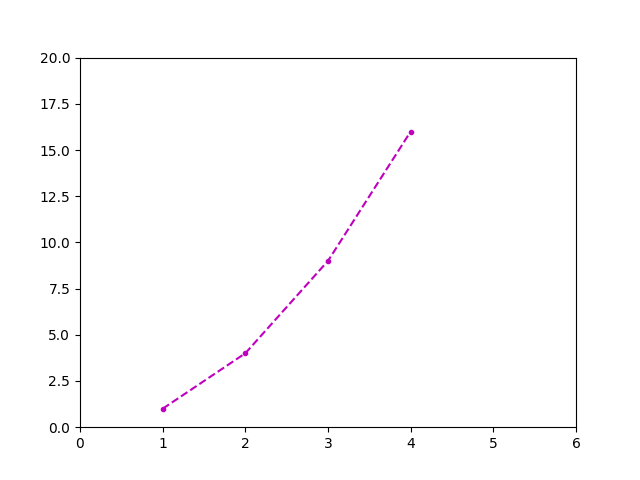
\includegraphics[width=0.5\textwidth]{matplotlib_magenta_markers}
    \caption{A plot with magenta markers}
    \label{fig:mpl_magenta_markers}
\end{figure}
\end{ex}

\func{pyplot.set_xlim(self, left=None, right=None, auto=False)}{Set the x axis limits}

\begin{ex}set\_xlim
\begin{lstlisting}[language=Python]
>>> set_xlim(left, right)
\end{lstlisting}
\begin{nb}
Passing limits in reverse order will flip the direction of the axis
\end{nb}
\begin{lstlisting}[language=Python]
>>> set_xlim(5000, 0)
\end{lstlisting}
\end{ex}

\func{pyplot.set_ylim(self, bottom=None, top=None, auto=False)}{Set the y axis limits}

\begin{ex}set\_ylim
\begin{lstlisting}[language=Python]
>>> set_ylim(bottom, top)
\end{lstlisting}
\begin{nb}
Passing limits in reverse order will flip the direction of the axis
\end{nb}
\begin{lstlisting}[language=Python]
>>> set_ylim(5000, 0)
\end{lstlisting}
\end{ex}

\subsubsection{Plotting with keyword strings}

Its often useful to have data in a format that allows for particular variables to be accessed. In Python dictionary objects are used, providing a key-value pair object. These can be used to plot categorical variables.

\begin{ex} Using the plot() data argument
\begin{lstlisting}[language=Python]
>>> kwdata = {'a': np.arange(50), 'b': np.random.randint(0, 50, 50)}
>>> plt.scatter('a', 'b', data=kwdata)
>>> plt.show()
\end{lstlisting}

\begin{figure}[h!]
    \centering
    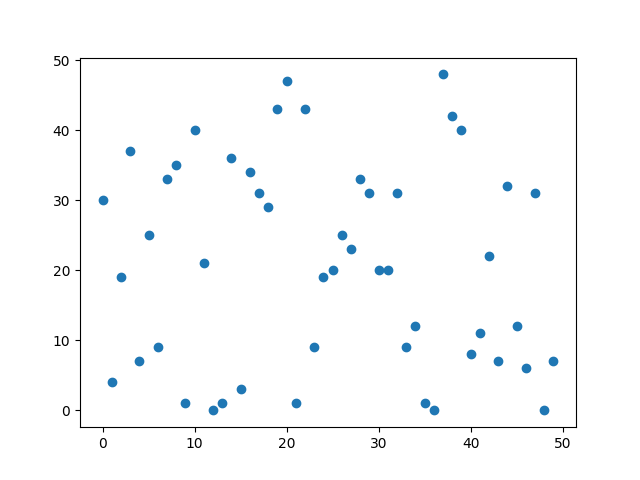
\includegraphics[width=0.5\textwidth]{matplotlib_using_kwdata}
    \caption{Plotting with keyword strings}
    \label{fig:mpl_kw}
\end{figure}
\end{ex}

\func{pyplot.scatter(x, y ,data=None, *args, **kwargs)}{Creates a scatter plot of y vs x with varying options}

\begin{nb}
plot function is faster for scatter plots when markers do not vary in size or color.
\end{nb}

\begin{nb}
fundamentally scatter plots work with 1D arrays
\end{nb}
\subsubsection{Plotting categorical variables}

\begin{ex}Plotting categorical variables
\begin{lstlisting}[language=Python]
>>> names = ['group_a', 'group_b', 'group_c']
>>> values = [1, 10, 100]
>>> plt.figure(figsize=(9, 3))
>>> plt.subplot(131)
>>> plt.bar(names, values)
>>> plt.subplot(132)
>>> plt.scatter(names, values)
>>> plt.subplot(133)
>>> plt.plot(names, values)
>>> plt.suptitle('Categorical Plotting')
>>> plt.show()
\end{lstlisting}

\begin{figure}[h]
    \centering
    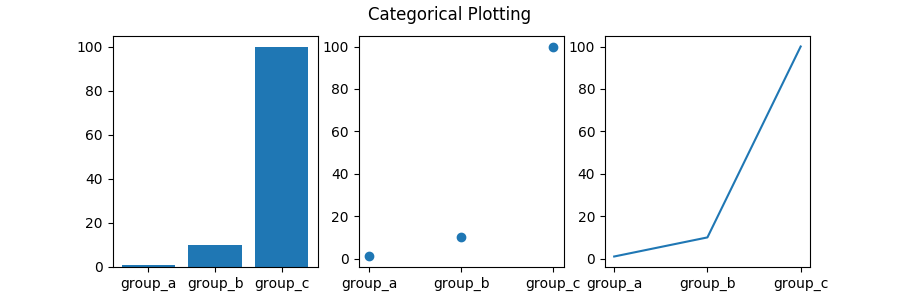
\includegraphics[width=\textwidth]{matplotlib_cat_vars}
    \caption{Plotting categorical variables}
    \label{fig:mpl_cat_vars}
\end{figure}
\end{ex}


\func{pyplot.subplot(*args, **kwargs)}{Adds a subplot to the current figure. Returns an \lstinline{Axes} object}


\begin{ex} subplot()
\begin{lstlisting}[language=Python]
plt.subplot(221)
ax1=plt.subplot(2, 2, 1) # equivalent
\end{lstlisting}
\end{ex}


\func{pyplot.suptitle(t, **kwargs)}{Adds a centred title to a figure}

\begin{nb}
Takes other parameters such as: \lstinline{horizontalalignment, verticalalignment , fontsize, fontweight} aliased by \lstinline{ha, va, size, weight}
\end{nb}

\subsubsection{Line Properties}

Lines under the \lstinline{matplotlib.lines.Line2D} class have many properties that can be set. 

\begin{table}[h!]
    \centering
    \begin{tabular}{ p{4cm} p{6cm}}
    \hline
    Property 	& 	Value Type \\
    \hline
    alpha 		& 	float \\ 
    animated 	& [True | False] \\
    antialiased or aa &	[True | False] \\
    clip\_box 	& a matplotlib.transform.Bbox instance \\
    clip\_on 	& [True | False] \\
    clip\_path 	& a Path instance and a Transform instance, a Patch \\
    color or c 	&	any matplotlib color \\
    contains 	& the hit testing function \\
    dash\_capstyle 	&	['butt' | 'round' | 'projecting'] \\
    dash\_joinstyle 	&	['miter' | 'round' | 'bevel'] \\
    dashes 		&	sequence of on/off ink in points \\
    data 		&	(np.array xdata, np.array ydata) \\
    figure 		&	a matplotlib.figure.Figure instance \\
    label 		&	any string \\
    linestyle or ls &	[ '-' | '--' | '-.' | ':' | 'steps' | ...] \\
    linewidth or lw &	float value in points \\
    marker 		&	[ '+' | ',' | '.' | '1' | '2' | '3' | '4' ] \\
    markeredgecolor or mec &	any matplotlib color \\
    markeredgewidth or mew &	float value in points \\
    markerfacecolor or mfc &	any matplotlib color \\
    markersize or ms &	float \\
    markevery 	&	[ None | integer | (startind, stride) ] \\
    picker 		&	used in interactive line selection \\
    pickradius 	&	the line pick selection radius \\
    solid\_capstyle 	&	['butt' | 'round' | 'projecting'] \\
    solid\_joinstyle &	['miter' | 'round' | 'bevel'] \\
    transform 	&	a matplotlib.transforms.Transform instance \\
    visible 	&	[True | False] \\
    xdata 		&	np.array \\
    ydata 		&	np.array \\
    zorder 		&	any number \\
    \hline
    \end{tabular}
\caption{Line2D Properties}
\label{table:line2d_props}
\end{table}


\subsubsection{Working with Text}


\func{pyplot.title(label, fontdict=None, loc='center', pad=None, **kwargs)}{Set a title for the axes.}

\begin{nb}
    The location or \lstinline{loc} can be set to one of \lstinline{center, left, right}\\
\end{nb}

\func{pyplot.xlabel(xlabel, fontdict=None, labelpad=None, **kwargs)}{Set the label for the x-axis.\\}

\func{pyplot.ylabel(ylabel, fontdict=None, labelpad=None)}{Set the label for the y-axis.\\}

\func{pyplot.text(x, y, s, fontdict=None, **kwargs)}{Add text to the axes. Where \lstinline{s} is the text, \lstinline{x, y} are data coordinates.\\}

\begin{nb}
    All the text commands returns a \lstinline{matplotlib.text.Text} instance.
\end{nb}


\begin{table}[h!]
    \centering
    \begin{tabular}{ p{4cm} p{8cm}}
	\hline
	Property & Value Type \\
	\hline
	alpha &	float \\
	backgroundcolor &	any matplotlib color \\
	color &	any matplotlib color \\
	horizontalalignment or ha &	[ 'center' | 'right' | 'left' ] \\
	label &	any string \\
	linespacing &	float \\
	name or fontname &	string e.g., ['Sans' | 'Courier' | 'Helvetica' ...] \\
	position &	(x, y) \\
	rotation &	[ angle in degrees | 'vertical' | 'horizontal' ] \\
	size or fontsize &	[ size in points | relative size, e.g., 'smaller', 'x-large' ] \\
	style or fontstyle &	[ 'normal' | 'italic' | 'oblique' ] \\
	variant &	[ 'normal' | 'small-caps' ] \\
	verticalalignment or va &	[ 'center' | 'top' | 'bottom' | 'baseline' ] \\
	visible &	bool \\
	weight or fontweight &	[ 'normal' | 'bold' | 'heavy' | 'light' | 'ultrabold' | 'ultralight'] \\
	x &	float \\
	y &	float \\
	\hline
    \end{tabular}
    \caption{Notable line properties}
    \label{tabel:mpl_line_props}
\end{table}

\begin{nb}
    \lstinline{matplotlib} accepts \TeX\ equation expressions in any text expression.
\end{nb}

\begin{ex}\TeX\ in \lstinline{matplotlib}
\begin{lstlisting}[language=Python]
plt.title(r'$\sigma_i=15$')
\end{lstlisting}
\end{ex}

\subsubsection{Annotating Text}

A common use for text is to annotate some feature of a plot. The \lstinline{annotate()} method provides help functionality to make annotations easy.\\

\func{pyplot.annotate(s, xy, *args, **kwargs)}{Annotates the point \lstinline{xy} with given text \lstinline{s}.}

\begin{nb}
    \lstinline{xy} is a tuple of floats \lstinline{(x, y})
\end{nb}

\begin{ex}Annotations
\begin{lstlisting}[language=Python]
t = np.arange(0.0, 5.0, 0.01)
s = np.cos(2*np.pi*t)
line, = plt.plot(t, s, lw=2)

plt.annotate('local max', xy=(2, 1), xytext=(3, 1.5), arrowprops=dict(facecolor='black', shrink=0.0))

plt.ylim(-2, 2)
plt.show()
\end{lstlisting}

\begin{figure}[h]
    \centering
    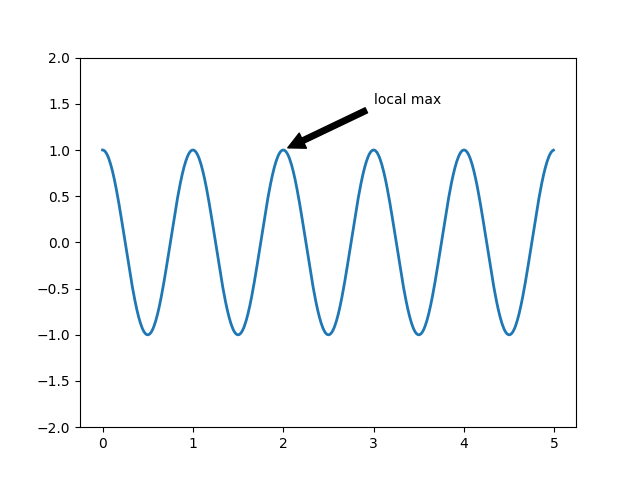
\includegraphics[width=\textwidth]{matplotlib_annotating_plots}
    \caption{Annotating a plot}
    \label{fig:mpl_ann}
\end{figure}
\end{ex}

\subsubsection{Non-linear Axes}

Matplotlib supports non linear, logarithmic and logit scales for axes. As well as the ability to create custom scales for plots; more information can be found in the \lstinline{matplotlib} docs.\\

\func{pyplot.yscale(value, **kwargs)}{Set the y-axis scale.\\}

\func{pyplot.xscale(value, **kwargs)}{Set the x-axis scale.\\}

\begin{nb}
Values that can be applied:

\begin{itemize}
    \item linear

    \item log

    \item symlog

    \item logit
\end{itemize}
\end{nb}

\hfill

\begin{ex}Non-linear axes
\begin{lstlisting}[language=Python]
y = np.random.normal(loc=0.5, scale=0.4, size=1000)
y = y[(y > 0) & (y < 1)]
y.sort()
x = np.arange(len(y))

# plot with various axes scales
plt.figure()

# linear
plt.subplot(121)
plt.plot(x, y)
plt.yscale('linear')
plt.title('linear')
plt.grid(True)

# log
plt.subplot(122)
plt.plot(x, y)
plt.yscale('log')
plt.title('log')
plt.grid(True)

plt.show()
\end{lstlisting}

\begin{figure}[h]
    \centering
    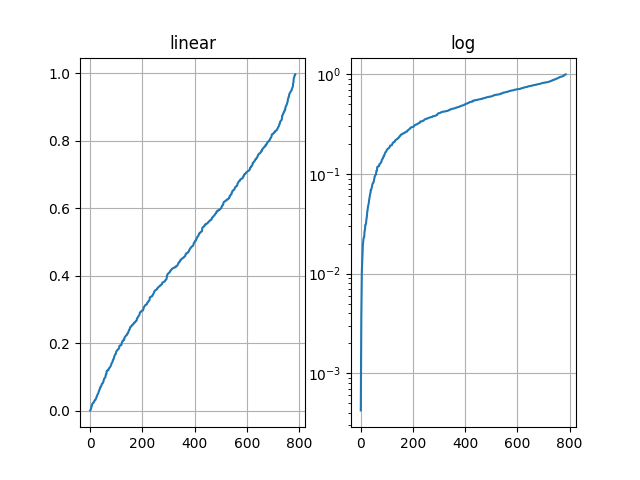
\includegraphics[width=\textwidth, height=8cm]{matplotlib_axis_scale}
    \caption{Changing the axis scale}
    \label{fig:mpl_axis_scale}
\end{figure}
\end{ex}


\break



\subsection{Images}

The matplotlib image module found under \lstinline{matplotlib.image} and typically imported as \lstinline{mpimg} supports basic image loading, rescaling and display operations.

\subsubsection{Importing image data into Numpy arrays}

Natively matplotlib only supports PNG images.\\

\func{image.imread(fname, format=None)}{Reads an image file into an numpy arra}

\begin{nb}
The returned shape of the array is either

\begin{itemize}
    \item \lstinline{(M, N)} for grey scale images

    \item \lstinline{(M, N, 3)} for RGB images

    \item \lstinline{(M, N, 4)} for RGBA images
\end{itemize}
\end{nb}

\begin{ex}Importing images
\begin{lstlisting}[language=Python]
>>> import matplotlib.image as mpimg
>>> img = mpimg.imread("./grasshopper.png")
>>> print(img)
[[0.40784314 0.40784314 0.40784314 ... 0.42745098 0.42745098 0.42745098]
 ...
 [0.44313726 0.4509804  0.4509804  ... 0.44705883 0.44705883 0.44313726]]
\end{lstlisting}
\end{ex}

\subsubsection{Plotting numpy arrays as images}

\func{pyplot.imshow(Arr, data=None, **kwargs)}{Display an image.}

\begin{rem}
    Colouring schemes are set by the \lstinline{cmap} parameter and include:
     \lstinline{"hot"},
     \lstinline{"jet"},
     \lstinline{"nipy_spectral"},
     \lstinline{"gnuplot"},
     \lstinline{"ocean"},
     as well as many others.
\end{rem}


\begin{ex}Display images
\begin{lstlisting}[language=Python]
>>> plt.imshow(img)
>>> plt.show()
\end{lstlisting}

\begin{nb}
A pseudocolour or false colour has been applied as the image is imported as a grey scale image with no colour set.
\end{nb}

\begin{figure}[H]
    \centering
    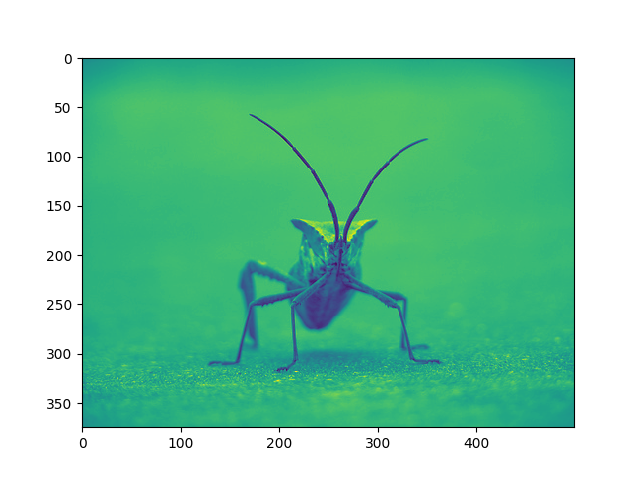
\includegraphics[width=0.7\textwidth]{matplotlib_img}
    \caption{Grasshopper}
    \label{fig:mpl_img}
\end{figure}
\end{ex}


\subsubsection{Colour scale reference}

\func{pyplot.colorbar(mappable=None, cax=None, ax=None, **kw)}{Adds a colorbar to a plot}

\begin{ex}Adding a colorbar
\begin{lstlisting}[language=Python]
>>> plt.imshow(img, cmap="gnuplot")
>>> plt.colorbar()
>>> plt.show()
\end{lstlisting}

\begin{figure}[H]
    \centering
    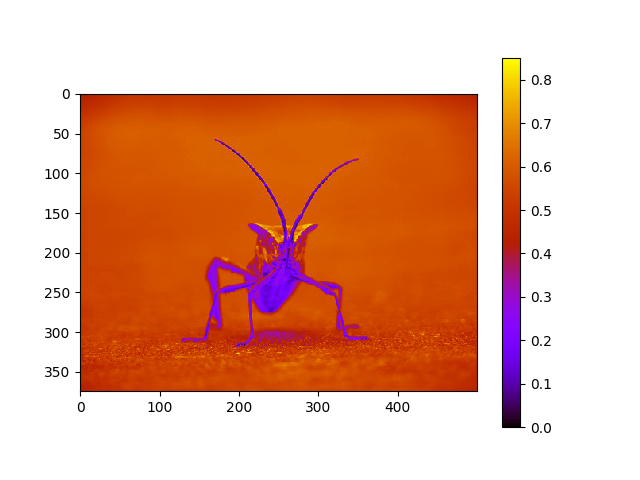
\includegraphics[width=0.7\textwidth]{matplotlib_col_bar}
    \caption{GNUplot \& colorbar}
    \label{fig:mpl_col_bar}
\end{figure}
\end{ex}


\subsubsection{Examining Image Data Ranges}

A useful tool to understand images in grater depth are histograms, we can visualise the range of colours in an image and in turn enhance the contrast, find important colours and so forth.\\

\func{pyplot.hist(x, bins=None, range=None, density=None, weights=None, cumulative=False, log=False, color=None, stacked=False}{Plot a histogram}

\begin{nb}
    There are boolean options like \lstinline{cumulative, density, log} \textit{etc.} used to change the histogram.
\end{nb}

\begin{ex}Examining images
\begin{lstlisting}[language=Python]
>>> plt.hist(img.ravel(), bins=256, range=(0.0, 1.0), fc="k")
>>> plt.show()
\end{lstlisting}


\begin{figure}[H]
    \centering
    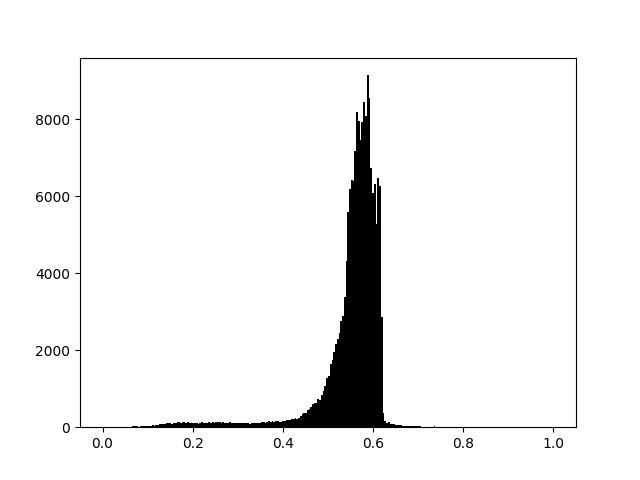
\includegraphics[width=0.7\textwidth]{matplotlib_exm_img}
    \caption{Grasshopper histogram}
    \label{fig:mpl_exm_img}
\end{figure}

\begin{rem}
    An interesting point is the peak at around 0.6. In order to look at the image within these limits more closely the \lstinline{clim} arg can be used.
\end{rem}
\end{ex}

\begin{ex}Setting a clim
\begin{lstlisting}[language=Python]
>>> plt.imshow(img, cmap="gnuplot", clim=(0, 0.6)))
\end{lstlisting}
\begin{figure}[H]
    \centering
    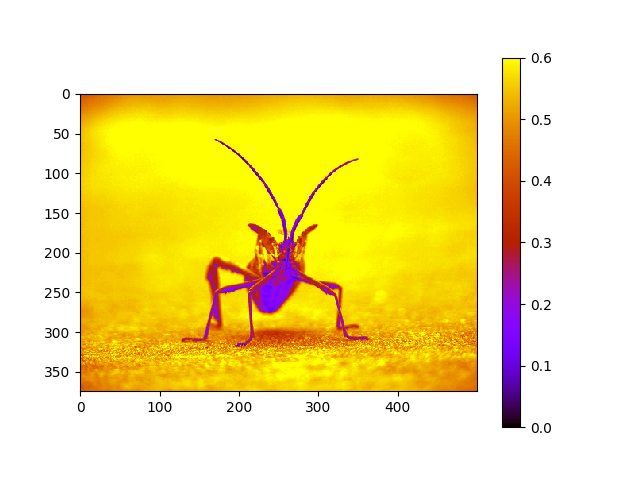
\includegraphics[width=0.7\textwidth]{matplotlib_ceil_img}
    \caption{Setting a clim}
    \label{fig:mpl_clim}
\end{figure}
\end{ex}


\break


\subsection{Interactive Mode}

Matplotlib has multiple backends that allow the user to work with images. When using OpenCV it is helpful to visually interpret whats happening to a plot as it happens, \textit{ex.} facial recognition, object detection and so on.\\

\func{pyplot.ion()}{Turns interactive mode on}

\begin{ex} Interactive mode
\begin{lstlisting}[language=Python]
>>> plt.ion()
>>> plt.plot([1, 2])
\end{lstlisting}
\begin{rem}
A window should appear with a plot being displayed
\end{rem}

\noindent The title can be set with:
\begin{lstlisting}[language=Python]
>>> plt.title("An interactive title")
\end{lstlisting}

\noindent and the title can be updated
\begin{lstlisting}[language=Python]
>>> plt.title("A new title")
\end{lstlisting}

\noindent For certain backends some functions require that the plot it explicitly drawn with:
\begin{lstlisting}[language=Python]
>>> plt.draw()
\end{lstlisting}
\end{ex}



\break




\section{OpenCV: Basics}

Typically the OpenCV namespace known as \lstinline{cv2} is imported as \lstinline{cv}.

\subsection{Images}

When working with images in OpenCV it is important to note that:

 \begin{enumerate}
    \item the following file types are supported: \lstinline{bmp, jpg, jp2, png, webp, pbm, pgm, ppm, pxm, ppm, st, pfm, tiff, tif, exr, hdr, pic}

    \item color images are decoded as \textbf{B G R} instead of RBG

    \item pixel length is limited to $ 2^{30} $

\end{enumerate}


\subsubsection{Reading Images}


\func{cv.imread(filename, flags=IMREAD_COLOR)}{Loads an image from a file.\\}

\noindent Flags can be found under the \lstinline{cv} namespace.
Available flags include:

\begin{table}[h!]
    \centering
    \def\arraystretch{1.1}%
    \begin{tabular}{ p{5.8cm} p{7cm}} 
    \hline
    Enumerator &  Description \\
    \hline
    \textbf{\footnotesize{IMREAD\_UNCHANGED}} & return the loaded image as is\\

    \textbf{\footnotesize{IMREAD\_GRAYSCALE}} & always convert image to the single channel grayscale \\

    \textbf{\footnotesize{IMREAD\_COLOR}} & always convert image to the 3 channel BGR \\

    \textbf{\footnotesize{IMREAD\_ANYDEPTH}} & return 16-bit/32-bit image \\

    \textbf{\footnotesize{IMREAD\_ANYCOLOR}} & the image is read in any possible color format. \\

    \textbf{\footnotesize{IMREAD\_LOAD\_GDAL}} & use the gdal driver for loading the image. \\

    \textbf{\footnotesize{IMREAD\_REDUCED\_GRAYSCALE\_2}} &convert image to single channel grayscale and reduce size by 1/2. \\

    \textbf{\footnotesize{IMREAD\_REDUCED\_COLOR\_2}} &  convert image to 3 channel BGR and reduce size by 1/2. \\

    \textbf{\footnotesize{IMREAD\_REDUCED\_GRAYSCALE\_4}} & convert image to single channel grayscale and reduce size by 1/4. \\

    \textbf{\footnotesize{IMREAD\_REDUCED\_COLOR\_4}} & convert image to  3 channel BGR and reduce size by 1/4. \\

    \textbf{\footnotesize{IMREAD\_REDUCED\_GRAYSCALE\_8}} & convert image to single channel grayscale and reduce size by 1/8. \\

    \textbf{\footnotesize{IMREAD\_REDUCED\_COLOR\_8}} & convert image to the 3 channel BGR and reduce size by 1/8. \\

    \textbf{\footnotesize{IMREAD\_IGNORE\_ORIENTATION}} & do not rotate the image\\
    \hline
    \end{tabular}
\end{table}

\break

\begin{ex} Reading an image
\begin{lstlisting}[language=Python]
import matplotlib.pyplot as plt
import numpy as np
import cv2 as cv


img = cv.imread("./grasshopper.png")

cv.imshow('grasshopper', img)
cv.waitKey(0)
cv.destroyAllWindows()
\end{lstlisting}

\noindent A window should appear with the specified image. In order to close the window and terminate the program any key can be pressed.
\end{ex}

\subsubsection{Useful functions for managing images}

\func{cv.imshow(winname, img)}{
Display an OpenGL 2D texture (img) in a specified window.\\
}

\func{cv.waitKey(delay=0)}{
Waits for a key to be pressed.
}
\begin{nb}
Delay of 0 means indefinitely; otherwise the time is in milliseconds.\\
\end{nb}

\func{cv.destroyAllWindows()}{
Destroys all the HighGUI windows.\\
}

\func{cv.destroyWindow(winname)}{
Destroys specified window.\\
}

\func{cv.imwrite(filename, img, *)}{
    Saves an image to a specified file
}

\begin{ex} Writing an image
\begin{lstlisting}[language=Python]
cv.imwrite('grasshopper.png',img)
\end{lstlisting}
\end{ex}

\subsubsection{Using Matplotlib}

There is an important distinction in the way matplotlib and OpenCV read images. Matplotlib reads images as RGB whereas OpenCV reads images as BGR. Therefore displaying an image that has been read with OpenCV in matplotlib or vice versa will result in the wrong colour representation.\\

To amend this issue either use the same library or if you import an image with OpenCV you can reverse the numpy array.\\

\begin{ex} Displaying images with matplotlib
\begin{lstlisting}[language=Python]
img = cv.imread('grasshopper.jpg')
img2 = img[:, :, ::-1]

# or

cv.cvtColor(img, cv.COLOR_BGR2RGB)
\end{lstlisting}
\end{ex}

\hfill

\begin{ex} Incorrectly displaying and image with matplotlib
\begin{lstlisting}[language=Python]
>>> img = cv.imread("./duck.webp")
>>> img2 = img[:, :, ::-1]
>>> plt.subplot(121)
>>> plt.imshow(img)
>>> plt.subplot(122)
>>> plt.imshow(img2)
>>> plt.show()
\end{lstlisting}
\begin{figure}[h!]
    \centering
    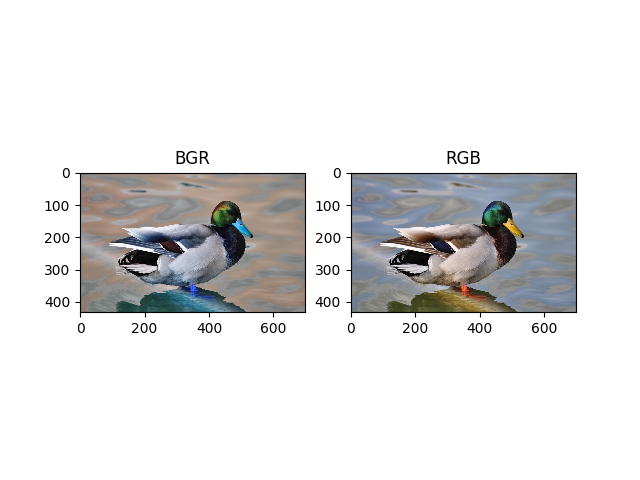
\includegraphics[width=\textwidth]{opencv_inv_cols}
    \caption{Inverted Colours}
    \label{fig:ocv_inv_cols}
\end{figure}


\end{ex}


\break


\subsection{Video}

\subsubsection{Capturing Video}

To capture video a \lstinline{VideoCapture} object is contructed.\\

\func{cv.VideoCapture}{
Class for capturing video from files, image sequences or cameras. The constuctor can either be passed a filename or an integer specifying which camera to use (starting from 0)
}

\begin{ex} Capturing Video
\begin{lstlisting}[language=Python]
cap = cv.VideoCapture(0)
if not cap.isOpened():
    print("Cannot open camera")
    exit()

while True:
    res, frame = cap.read() # combines cap.grab() and cap.retrieve()

    if not res:
        print("Can't receive frame")
        break

    gray_frame = cv.cvtColor(frame, cv.COLOR_BGR2GRAY)
    cv.imshow('frame', gray_frame) # display

    if cv.waitKey(1) == ord('q'):
        break

cap.release() # close capture stream
cv.destroyAllWindows()
\end{lstlisting}
\end{ex}


\subsubsection{\lstinline{VideoCapture} methods}

\hfill

\func{VideoCapture.isOpened()}{
Returns true if the video capturing has been initalized already.\\
}

\func{VideoCapture.grab()}{
Grabs the next frame in the video file or capturing device. Returns true in case of success.\\
}

\func{VideoCapture.retrieve()}{
Decodes and returns the grabbed video frame.\\
}

\func{VideoCapture.read()}{
Grabs, decodes and returns the next video frame. Returns false if no frame has been grabbed. Shorthand for calling both \lstinline{grab} and \lstinline{retrieve}.\\
}

\func{VideoCapture.release()}{
Closes the video file or capturing device.\\
}

\func{VideoCapture.get(propId)}{
Returns the specified VideoCapture property.\\
}

\func{VideoCapture.set(propId, value)}{
Sets a property in the VideoCapture.\\
}


\begin{table}[h!]
    \centering
    \def\arraystretch{1.1}%
    \begin{tabular}{ p{5cm} p{7cm} } 
    \hline
    Enumerator &  Description \\
    \hline
    \textbf{\footnotesize{CAP\_PROP\_POS\_MSEC}} & Current position of the video file in milliseconds \\

    \textbf{\footnotesize{CAP\_PROP\_POS\_FRAMES}} & 0-based index of the frame to be decoded/captured next \\

    \textbf{\footnotesize{CAP\_PROP\_FRAME\_WIDTH}} & Width of the frames in the video stream \\

    \textbf{\footnotesize{CAP\_PROP\_FRAME\_HEIGHT}} & Height of the frames in the video stream \\

    \textbf{\footnotesize{CAP\_PROP\_FPS}} & Frame rate \\

    \textbf{\footnotesize{CAP\_PROP\_FRAME\_COUNT}} & Number of frames in the video file \\

    \textbf{\footnotesize{CAP\_PROP\_FORMAT}} & Format of the Mat objects returned by VideoCapture::retrieve() \\

    \textbf{\footnotesize{CAP\_PROP\_BRIGHTNESS}} & Brightness of the image \\

    \textbf{\footnotesize{CAP\_PROP\_CONVERT\_RGB}} & Boolean flags indicating whether images should be converted to RGB \\
    \hline
    \end{tabular}
    \caption{Commonly Used VideoCapture properties}
    \label{table:ocv_vca_props}
\end{table}

\subsubsection{Reading Video from file}

Reading videos from file can uses the \lstinline{VideoCapture} class. 

\begin{ex}Reading Videos from File
\begin{lstlisting}[language=Python]

cap = cv.VideoCapture("./video.mp4")

while True:
    res, frame = cap.read() # combines cap.grab() and cap.retrieve()

    if not res:
        break

    gray_frame = cv.cvtColor(frame, cv.COLOR_BGR2GRAY)
    cv.imshow('frame', gray_frame) # display

    if cv.waitKey(1) == ord('q'):
        break
...
\end{lstlisting}
\begin{nb}
    Videos do not play back seems faster than intended. This is because there is no limit to how many frames can be played a seconds. It may be interesting to wait for $ fps^{-1} $ seconds between frames.
\end{nb}
\end{ex}

\subsubsection{Writing Video}

The \lstinline{VideoWriter} class is ueed to wite (save) videos.\\ 

\func{cv.VideoWriter(filename, fourcc, fps, size, isColor=True}{
Initializes a video writer.\\
}

\begin{df}FourCC (four-character code)

A sequence of four bytes used to identify data formats. In terms of OpenCV the 4 char code is used to compress the frames.\\

\noindent Some character codes include: \lstinline{DIVX, XVID, X264, WMV1, MJPG}
\end{df}

\begin{nb}
    A FourCC code can be obtained via \lstinline{cv.VideoWriter.fourcc(*'XVID')}
\end{nb}
   

\begin{ex}Writing Video
\begin{lstlisting}[language=Python]
cap = cv.VideoCapture(0)
fourcc = cv.VideoWriter.fourcc(*"XVID")
out = cv.VideoWriter('output.avi', fourcc, 20.0, (640,  480))

while cap.isOpened():
    ret, frame = cap.read()
    if not ret:
        print("Can't receive frame")
        break

    frame = cv.flip(frame, 1) # vertically flips image

    out.write(frame)
    cv.imshow('frame', frame)
    if cv.waitKey(1) == ord('q'):
        break

cap.release()
out.release()
cv.destroyAllWindows()
\end{lstlisting}
\end{ex}
   
\func{cv.flip(frame, flipCode)}{
Flips a 2D array around horizontal, vertical or both axes.\\

\noindent flipCode $ < 0 $ flips both axes \\
flipCode $ = 0 $ flips horizontally \\
flipCode $ > 0 $ flip vertically \\
}

\subsubsection{\lstinline{VideoWriter} methods}

\func{VideoWriter.open()}{
    Initializes or reinitializes the video writer. Returns \lstinline{true} if successful.\\

}

\func{VideoWriter.isOpened()}{
    Returns \lstinline{true} if video writer successfully Initialized.\\
}

\func{VideoWriter.release()}{
Closes the video writer.\\
}

\func{VideoWriter.write(img)}{
Writes the next video frame.\\
}

\func{VideoWriter.getBackendName()}{
Returns used backend API.\\
}


\func{VideoWriter.set(propId, val)}{
    Sets a \lstinline{VideoWriter} property\\
}


\func{VideoWriter.get()}{
    Returns the specified \lstinline{VideoWriter} property.\\
}

\begin{table}[h!]
    \centering
    \def\arraystretch{1.1}%
    \begin{tabular}{ p{5cm} p{7cm} } 
    \hline
    Enumerator &  Description \\
    \hline
    \textbf{\footnotesize{VIDEOWRITER\_QUALITY}} & Current quality (0..100\%) of the encoded videostream. Can be adjusted dynamically in some codecs \\

    \textbf{\footnotesize{VIDEOWRITER\_FRAMEBYTES}} & (Read-only): Size of just encoded video frame. Note that the encoding order may be different from representation order \\

    \textbf{\footnotesize{VIDEOWRITER\_NSTRIPES}} & Number of stripes for parallel encoding. -1 for auto detection \\
    \hline
    \end{tabular}
    \caption{\lstinline{VideoWriter} properties}
    \label{table:ocv_vca_props}
\end{table}


\break


\subsection{Drawing Functions}

All drawing classes, functions and enumerations in OpenCV are found under \lstinline{Imgproc_draw} and are imported into the main \lstinline{cv2} namespace.

\subsubsection{Lines}

\func{cv.line(img, pt1, pt2, col, thickness, shift=0}{
Draws a line connecting two points \lstinline{pt1, pt2}
}

\begin{ex} Drawing Lines
\begin{lstlisting}[language=Python]
img = np.full((512, 512, 3), 251.0)
cv.line(img, (0, 0), (511, 511), (255, 0, 0), 2)
cv.line(img, (511, 0), (0, 511), (0, 0, 255), 2)
\end{lstlisting}

\begin{figure}[h!]
    \centering
    
\includegraphics[width=0.5\textwidth]{opencv_lines}
    \caption{Drawing Lines}
    \label{fig:ocv_drw_lin}
\end{figure}

\end{ex}

\begin{rem}
    When plottings lines or more generally when dealing with images, the \textbf{top left} pixel is point $ (0, 0) $. 
\end{rem}


\begin{figure}[h!]
    \centering
    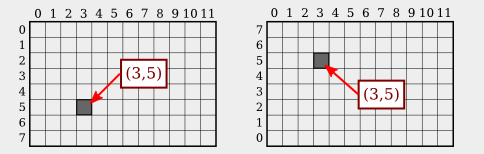
\includegraphics[width=0.83\textwidth]{computer_graphics}
    \caption{Computer Graphics}
    \label{fig:comp_graph}
\end{figure}

\subsubsection{Rectangles}

\func{cv.rectangle(img, pt1, pt2, col, thickness=1, lineType=LINE_0, shift=0)}{
Draws a rectangle, negative thickness means the rectangle will be filled.
}

\begin{ex}Drawing Rectangles
\begin{lstlisting}[language=Python]
img = np.full((512, 512, 3), 251.0)
cv.rectangle(img, (63, 63), (447, 447), (0, 255, 0), -1)
\end{lstlisting}


\begin{figure}[h!]
    \centering
    
\includegraphics[width=0.5\textwidth]{opencv_rect}
    \caption{Drawing Rectangles}
    \label{fig:ocv_drw_rct}
\end{figure}
\end{ex}

\subsubsection{Circles}

\func{cv.circle(ing, center, rad, col, thickness=1, lineType=LINE_0, shift=0)}{
Draws a circle with a given center and radius
}

\begin{ex} Drawing Circles
\begin{lstlisting}[language=Python]
cv.circle(img, (255, 255), 128, (0, 255, 100), 2)
\end{lstlisting}
\end{ex}


\subsubsection{Ellipses}

\func{cv.ellipse(ing, center, axes, rotation, startAngle, endAngle, col, thickness=1, lineType=LINE_0, shift=0)}{
Draws an ellipse, can be filled by changing the line type. 
}

\begin{ex} Drawing Ellipses
\begin{lstlisting}[language=Python]
cv.ellipse(img, (255, 255), 
		(100, 200), # axes
		0, 90, 320, # rotation, start, end
		(0, 0, 255), -1)
\end{lstlisting}
\begin{figure}[h!]
    \centering
    
\includegraphics[width=0.5\textwidth]{opencv_elip}
    \caption{Drawing Ellipses}
    \label{fig:ocv_drw_eli}
\end{figure}
\end{ex}

\subsubsection{Polygons}

\func{cv.polylines(img, *pts, isClosed, col, thickness,... )}{Draws several polygoonal curves.}


\begin{ex} Drawing Polygons
\begin{lstlisting}[language=Python]
points = np.array([(63,63), (447, 127), (63, 195), (447, 255), (63, 319), (447, 383)], np.int32)
points = points.reshape((-1, 1, 2))
cv.polylines(img, [points], True, 255, 1)
\end{lstlisting}
\begin{figure}[h!]
    \centering
    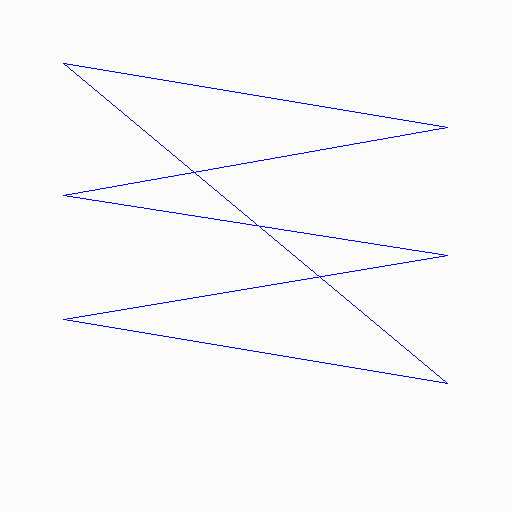
\includegraphics[width=0.5\textwidth]{opencv_polylines}
    \caption{Drawing Polygons}
    \label{fig:ocv_drw_pli}
\end{figure}
\end{ex}


\subsubsection{Text}

\func{cv.putText(img, text, org, fontFace, fontScale, col, thickness=1, lineType=LINE_0, bottomLeftOrigin=False)}{Draws a text string. Symbols that cannot be rendered are replaced by question marks.}

\begin{ex} Drawing Text
\begin{lstlisting}[language=Python]
font = cv.FONT_HERSHEY_SIMPLEX
cv.putText(img, "oCV", (200, 300), font, 2, (0, 0, 0), 2,cv.LINE_AA)
\end{lstlisting}
\begin{figure}[h!]
    \centering
    
\includegraphics[width=0.5\textwidth]{opencv_text}
    \caption{Drawing Text}
    \label{fig:ocv_drw_txt}
\end{figure}
\end{ex}

\subsubsection{Miscellaneous}

\func{cv.arrowLine(img, pt1, pt2, col, thickness=1, tipLength=0.1)}{Draws an arrow segments pointing from pt1 to pt2.\\}

\func{cv.drawMarker(img, pt, col, markerType=MARKER_CROSS, markerSize=20)}{Draws a marker at a given point.\\}

\func{cv.drawContours(img, *contours, countourIdx, col, thickness=1, hierarchy=[], maxLevel, offset)}{Draws contours outlines or filled contours.\\}


\break


\subsection{GUIs}

Graphical user interfaces or GUIs are constructed with the \lstinline{highgui} module. The module is responsible for: creating and managing windows, creating GUI elements mainly trackbars and dealing with window interactions such as mouse events.

\subsubsection{Creating Windows}

\func{cv.namedWindow(winname, flags=WINDOW_AUTOSIZE)}{Creates a window that can be used as a place holder for images and track bars.\\}

\begin{nb}
If a window with the same name exists the function does nothing.
\end{nb}

\begin{table}[h!]
    \centering
    \def\arraystretch{1.1}%
    \begin{tabular}{ p{5cm} p{7cm} } 
	\hline
	Enumerator & Description \\
	\hline
	\textbf{\footnotesize{WINDOW\_NORMAL}} & window can be resized \\

	\textbf{\footnotesize{WINDOW\_ AUTOSIZE}} & window cannot be resized, size determined by the image being displayed \\

	\textbf{\footnotesize{WINDOW\_OPENGL}} & window with opengl support \\

	\textbf{\footnotesize{WINDOW\_FULLSCREEN}} & fullscreen window \\

	\textbf{\footnotesize{WINDOW\_FREERATIO}} & the image expends as much as it can (no ratio constraint) \\

	\textbf{\footnotesize{WINDOW\_KEEPRATIO}} & the ratio of the image is respected \\

	\textbf{\footnotesize{WINDOW\_GUI\_EXPANDED}} & window with status bar and tool bar \\

	\textbf{\footnotesize{WINDOW\_GUI\_NORMAL}} & old fashioned way, not recommended \\
    \hline
    \end{tabular}
    \caption{Window Flags}
    \label{table:win_flgs}
\end{table}

\func{cv.resizeWindow(winname, width, height)}{Resizes window to the specified size.\\}

\func{cv.moveWindow(winname, x, y)}{Moves window to the specified position.\\}

\func{cv.setWindowTitle(winname, title)}{Updates window title.\\}

\func{cv.setWindowProperty(winname, prop_id, prop_value)}{Changes parameters of a window dynamically.\\}

\func{cv.getWindowProperty(winname, prop_id)}{Provides parameters of a window.\\}

\subsubsection{Mouse Events}

OpenCV can be used to listen for mouse events. In order for OpenCV to interact with mouse data, the \lstinline{setMouseCallback} function and a callback function are needed.

\begin{df}Callback Function

A function that is passed into another function as an argument and is invoked inside the outer function to complete some kind of action.
\end{df}


\func{cv.setMouseCallback(winame, onMouse, userdata=0)}{Sets mouse handler for the specified window. \lstinline{onMouse} is a callback function for mouse events.\\}

\func{cv.MouseCallback(event, x, y, flags, userdata)}{Callback function for mouse events.\\}

\noindent Available mouse events include:

\begin{table}[h!]
    \centering
    \def\arraystretch{1.1}%
    \begin{tabular}{ p{5cm} p{7cm} } 
	\hline
	Enumerator & Description \\
	\hline
	\textbf{\footnotesize{EVENT\_MOUSEMOVE}} & indicates that the mouse pointer has moved over the window \\
	
	\textbf{\footnotesize{EVENT\_LBUTTONDOWN}} & indicates that the left mouse button is pressed \\
	
	\textbf{\footnotesize{EVENT\_RBUTTONDOWN}} & indicates that the right mouse button is pressed \\
	
	\textbf{\footnotesize{EVENT\_MBUTTONDOWN}} & indicates that the middle mouse button is pressed \\
	
	\textbf{\footnotesize{EVENT\_LBUTTONUP}} & indicates that left mouse button is released \\
	
	\textbf{\footnotesize{EVENT\_RBUTTONUP}} & indicates that right mouse button is released \\
	
	\textbf{\footnotesize{EVENT\_MBUTTONUP}} & indicates that middle mouse button is released \\
    
	\textbf{\footnotesize{EVENT\_LBUTTONDBLCLK}} & indicates that left mouse button is double clicked \\
	
	\textbf{\footnotesize{EVENT\_RBUTTONDBLCLK}} & indicates that right mouse button is double clicked \\
	
	\textbf{\footnotesize{EVENT\_MBUTTONDBLCLK}} & indicates that middle mouse button is double clicked \\
	
	\textbf{\footnotesize{EVENT\_MOUSEWHEEL}} & positive and negative values mean forward and backward scrolling, respectively \\
	
	\textbf{\footnotesize{EVENT\_MOUSEHWHEEL}} & positive and negative values mean right and left scrolling, respectively \\
	\hline
    \end{tabular}
    \caption{Mouse Events}
    \label{table:mouse_events}
\end{table}

\break

\begin{ex} Mouse Events
\begin{lstlisting}[language=Python]
img = np.full((512, 512, 3), 251.0)
cv.namedWindow('image')

def draw_circle(event, x, y, flags, userdata):
    ''' Callback function that draws a circle '''
    if event == cv.EVENT_LBUTTONDBLCLK:
        cv.circle(img, (x, y), 100, (255, 0, 0), 1)

cv.setMouseCallback('image', draw_circle)

while(True):
    cv.imshow('image', img)
    if cv.waitKey(20) & 0xFF == 27: # esc key
        break

cv.destroyAllWindows()
\end{lstlisting}
\begin{nb}
When there is a change in the state of the mouse, the callback if fired containing information such as \lstinline{x, y} position, the \lstinline{event} and additional \lstinline{flags}.\\
\end{nb}
\end{ex}

\noindent Event flags can be used to narrow down events even further. Available flags include: \\

\begin{table}[h!]
    \centering
    \def\arraystretch{1.1}%
    \begin{tabular}{ p{5cm} p{7cm} } 
	\hline
	Enumerator & Description \\
	\hline
	\textbf{\footnotesize{EVENT\_FLAG\_LBUTTON}} & indicates that the left mouse button is down \\

	\textbf{\footnotesize{EVENT\_FLAG\_RBUTTON}} & indicates that the right mouse button is down \\

	\textbf{\footnotesize{EVENT\_FLAG\_MBUTTON}} & indicates that the middle mouse button is down \\

	\textbf{\footnotesize{EVENT\_FLAG\_CTRLKEY}} & indicates that CTRL Key is pressed \\

	\textbf{\footnotesize{EVENT\_FLAG\_SHIFTKEY}} & indicates that SHIFT Key is pressed \\

	\textbf{\footnotesize{EVENT\_FLAG\_ALTKEY}} & indicates that ALT Key is pressed \\
	\hline
    \end{tabular}
    \caption{Event Flags}
    \label{table:event_flags}
\end{table}


\subsubsection{Trackbars}

Trackbars are an extremely useful tool for quickly interacting with a range of values. They can be used to change image properties such as brightness, function parameters such as drawing function colours etc. Trackbars are created using the \lstinline{createTrackbar} function.\\

\func{cv.createTrackbar(trackbarname, winname, val, count, onChange=0, data=0)}{Creates a trackbar and attaches it to the specified window. \lstinline{value} is the initial value of the trackbar.}

\func{cv.TrackbarCallback(pos, userdata)}{Callback function for Trackbar.\\}

\noindent Much like Mouse Events trackbars also require a callback.\\

\begin{ex}Using Trackbars
\begin{lstlisting}[language=Python]
...
def draw_circle(event, x, y, flags, params):
    ''' Callback function that draws a circle '''
    if event == cv.EVENT_LBUTTONDBLCLK:
        red = cv.getTrackbarPos("R", "image")
        thickness = cv.getTrackbarPos("T", "image")
        cv.circle(img, (x, y), 100, (0, 0, red), thickness)

def empty_func(x): pass

cv.createTrackbar("R", "image", 122, 255, empty_func)
cv.createTrackbar("T", "image", 5, 50, empty_func)
cv.setMouseCallback('image', draw_circle)
...
\end{lstlisting}
\end{ex}

\noindent Some additional function for interacting with trackbars:\\


\func{cv.getTrackbarPos(trackbarname, winname)}{Returns the position of the trackbar.\\}

\func{cv.setTrackbarPos(trackbarname, winame, pos)}{Set the trackbar position.\\}

\func{cv.setTrackbarMax(trackbarname, winname, maxval)}{Set the trackbar maximum position.\\}

\func{cv.setTrackbarMin(trackbarname, winname, minval)}{Set the trackbar minimum position.\\}




\break


\section{OpenCV: Image Processing}

Image processing plays a fundamental role in OpenCV, before information can be extracted from an image about say the location of an object, the presence of a face etc. An image must be manipulated in such way that removes unnecessary information or enhances existing information. Therefore, images need to be combined, noise removed, motion de-blurred and so on. The following section explores the available options for processing images in OpenCV.

\subsection{Colour Space}

\begin{df} Colour Space

An abstract mathematical model that describes colours. They are also referred to as colour models.
\end{df}


\subsubsection{HSV Colour Space}

HSV stands for Hue, Saturation, Visibility. It is a commonly used colour space and provides a more natural way or thinking about colour. Rather than RGB / BGR which considers colour as a combinations of the three primary colours.

\begin{figure}[h!]
    \centering
    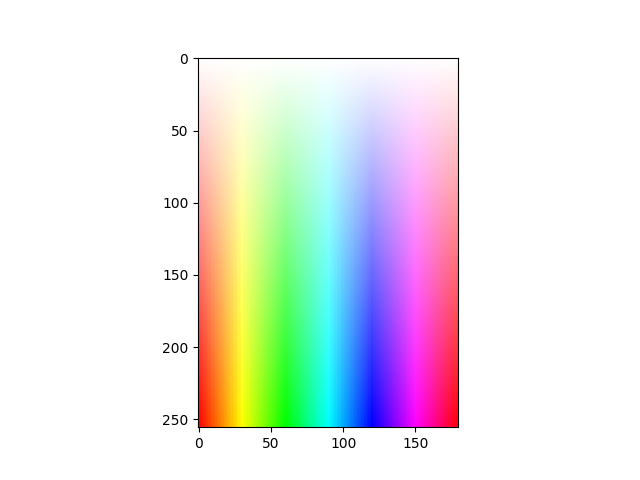
\includegraphics[width=\textwidth]{HSV_col_space}
    \caption{HSV Colour Space}
    \label{fig:hsv_cls}
\end{figure}

\begin{nb}
    The visibility is constant in this case, however it can be thought of as the amount of darkness / greyness in the image. A low visibility means that the colour is darker.
\end{nb}

\noindent The range for each value in OpenCV is:
\begin{itemize}
    \item H $ [0, 179] $
    \item S $ [0, 255] $
    \item V $ [0, 255] $
\end{itemize}

\subsubsection{Changing Colour Space}

The \lstinline{cvtColor} function is used to convert between colour spaces.\\

\func{cvtColor(img, dst, code}{Converts an image from one colour space to another.\\}


\begin{ex}Converting BGR TO HSV
\begin{lstlisting}[language=Python]
duck = cv.imread("./duck.png")
hsv_duck = cv.cvtColor(duck, cv.COLOR_BGR2HSV)
cv.imshow("image", hsv_duck)
\end{lstlisting}

\begin{nb}
The image has been converted to HSV however is being displayed in BGR; appearing unusual.
\end{nb}
\end{ex}

\begin{table}[h!]
    \centering
    \def\arraystretch{1.1}%
    \begin{tabular}{ p{5cm} p{7cm} } 
	\hline
	Conversion & Description \\
	\hline
	\textbf{\footnotesize{COLOR\_BGR2GRAY}} & BGR and grayscale \\

	\textbf{\footnotesize{COLOR\_BGR2BGR565}} & BGR and BGR565 (16-bit images)  \\

	\textbf{\footnotesize{COLOR\_GRAY2BGR565}} & grayscale to BGR565 (16-bit images)  \\

	\textbf{\footnotesize{COLOR\_BGR2XYZ}} & BGR to CIE XYZ \\

	\textbf{\footnotesize{COLOR\_BGR2YCrCb}} & BGR to luma-chroma (aka YCC) \\

	\textbf{\footnotesize{COLOR\_BGR2HSV}} & BGR to HSV (hue saturation value) \\

	\textbf{\footnotesize{COLOR\_BGR2Lab}} & BGR to CIE Lab \\

	\textbf{\footnotesize{COLOR\_BGR2Luv}} & BGR to CIE Luv \\

	\textbf{\footnotesize{COLOR\_BGR2HLS}} & BGR to HLS (hue lightness saturation) \\
	\hline
    \end{tabular}
    \caption{Colour Space Conversions}
    \label{table:col_convs}
\end{table}

\begin{rem}
There are over 150 colour conversions available.\\

\begin{lstlisting}[language=Python]
>>> [print(i) for i in dir(cv) if i.startswith('COLOR_')]
\end{lstlisting}
Prints the available conversions
\end{rem}


\break


\subsection{Image Arithmetic}

Image arithmetic applies the standard arithmetic operations or logical operators to two or more images. Operators are applied on a pixel by pixel basis, therefore the value of the pixel is dependant only on the corresponding image pixel value. Typically logical operators are applied on binary (black and white) images, in order to combine or remove elements.\\

\noindent  Throughout the example the following image will be used
\begin{lstlisting}[language=Python]
ints = np.array([(127, 63), (63, 191), (191, 191)],np.int32)
points.reshape((-1, 1, 2))

triangle = cv.fillPoly(np.zeros((255, 255), np.uint8), [points], 170)
rectangle = cv.rectangle(np.zeros((255, 255), np.uint8), (63, 63), (191, 191), 80, -1)
\end{lstlisting}


\subsubsection{Addition}

Addition is performed element wise

\begin{equation}
    Q(i, j) = P_1(i, j) + P_2(i, j)\\
\end{equation}\\

\noindent Alternatively pixel value can be added to a constant $ C $:

\begin{equation*}
    Q(i, j) = P_1(i, j) + C
\end{equation*}

\begin{ex} Addition
\begin{lstlisting}[language=Python]
rectangle + triangle
rectangle + 100
\end{lstlisting}
\begin{figure}[h!]
    \centering
    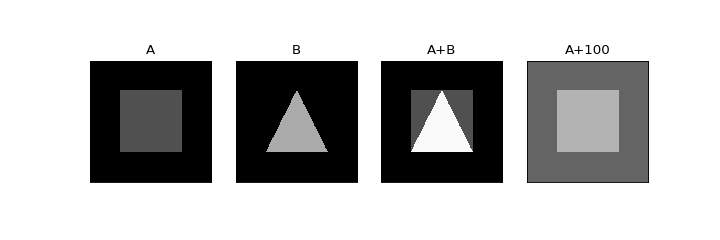
\includegraphics[width=\textwidth]{ocv_addition}
    \caption{Addition}
    \label{fig:ocv_add}
\end{figure}
\end{ex}


\subsubsection{Subtraction}

Pixel subtraction  takes two images and produces an output image whose pixels values are those of the first image minus the corresponding pixel values from the second image. It is also possible to subtract a constant from the image.

\begin{equation}
    Q(i, j) = P_1(i, j) - P_2(i, j)\\
\end{equation}\\

\noindent Alternatively a constant $ C $ can be subtracted:

\begin{equation*}
    Q(i, j) = P_1(i, j) - C
\end{equation*}

\begin{ex} Subtraction
\begin{lstlisting}[language=Python]
# Rectangle an Traingle pixel values changed to 200
rectangle - triangle
rectangle - 200
\end{lstlisting}
\begin{figure}[h!]
    \centering
    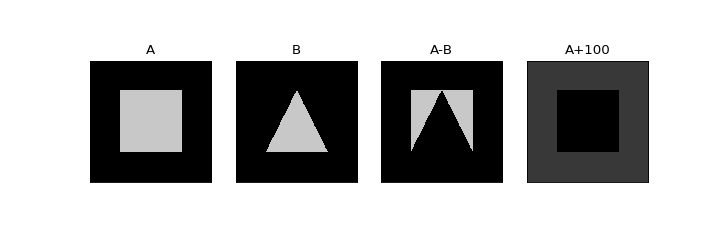
\includegraphics[width=\textwidth]{ocv_subtraction}
    \caption{Subtraction}
    \label{fig:ocv_sub}
\end{figure}
\end{ex}

\begin{rem}
Implementations of the operator vary as to what it does if the output pixels are negative. For instance a pixel value of $ -30 $ appears as $ 226 $ 
\end{rem}

Image subtraction can be useful for removing uneven lighting in an image. For instance in microscopy; an image may be taken when the lighting is poor of some item, a similar image can be taken without the item but with the same uneven light source, subtracting one image from the other would result in a darker but evenly lit image.


\subsubsection{Multiplication}

Similar to other arithmetic operations pixel multiplication can consist of multiplying one pixel value by another, or multiplying by a constant.


\begin{equation}
    Q(i, j) = P_1(i, j) \times P_2(i, j)\\
\end{equation}\\

\begin{equation*}
    Q(i, j) = P_1(i, j) \times C
\end{equation*}

\begin{ex} Multiplication
\begin{lstlisting}[language=Python]
rectangle * 0.5
triangle  * 1.5
\end{lstlisting}
\begin{figure}[h!]
    \centering
    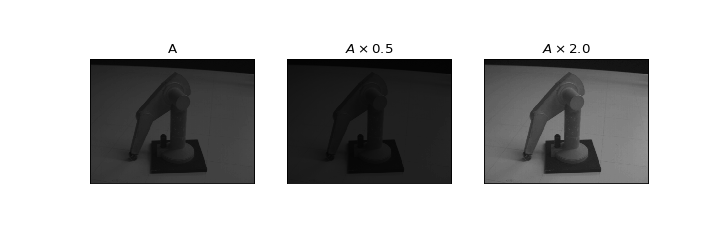
\includegraphics[width=\textwidth]{ocv_multiplication}
    \caption{Multiplication}
    \label{fig:ocv_mult}
\end{figure}
\end{ex}


\begin{rem}
Pixel multiplication can come in useful when trying to increase / decrease the brightness of an image. For instance a scaling factor $ C > 1 $ would increase the brightness, and a factor $ C < 1 $ would decrease the brightness.
\end{rem}

\begin{nb}
Using pixel multiplication often gives better results than just adding the same value to each pixel as the relative contrast of the image is preserved.
\end{nb}

\subsubsection{Division}

Image division take two images as input and produces a third image whose pixel values are the pixel values of the first image divided by the corresponding values in the second image.

\begin{equation}
    Q(i, j) = \frac{P_1(i, j)}{P_2(i, j)}
\end{equation}\\

\begin{equation*}
    Q(i, j) = \frac{P_1(i, j)}{C}
\end{equation*}

One of the most important uses of division is in change detection. This is similar to subtraction but instead of giving the absolute change for each pixel from one to the next, it gives the ratio between corresponding pixel values.\\

\begin{ex} Division
\begin{lstlisting}[language=Python]
div1 = cv.imread("./images/division1.png", 0)
div2 = cv.imread("./images/division2.png", 0)
(div1 / div2) * 100) # scaled for visibility
\end{lstlisting}
\begin{figure}[h!]
    \centering
    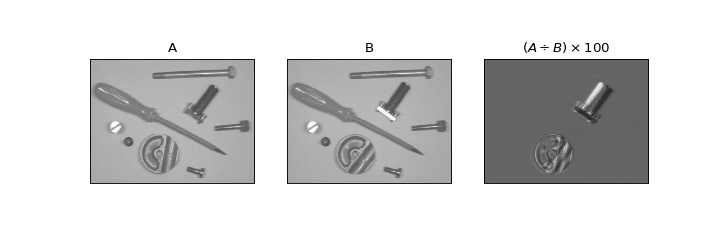
\includegraphics[width=\textwidth]{ocv_division}
    \caption{Division}
    \label{fig:ocv_division}
\end{figure}
\end{ex}


\subsubsection{Logical AND}

The AND operator takes in two images and determines the values of the third images pixels based on the following truth table:

\begin{table}[H]
    \centering
    \def\arraystretch{1.1}%
    \begin{tabular}{ c c c } 
	\hline
	A & B & Q \\
	\hline
	0 & 0 & 0 \\
	0 & 1 & 0 \\
	1 & 0 & 0 \\
	1 & 1 & 1 \\
	\hline
    \end{tabular}
\end{table}

\noindent Mathematically the operator is defined as:

\begin{equation}
    Q(i,j) = P_1(i, j) \land P_2(i, j) 
\end{equation} \\

\func{np.logical_and(x1, x2)}{Computes the truth value of x1 AND x2 element-wise.}

\begin{ex} AND
\begin{lstlisting}[language=Python]
circle_r = cv.circle(np.zeros((255, 255), np.uint8), (159, 127), 64, 255, -1)
circle_l = cv.circle(np.zeros((255, 255), np.uint8), (93, 127), 64, 255, -1)

np.logical_and(circle_r, circle_l)
\end{lstlisting}
\begin{figure}[H]
    \centering
    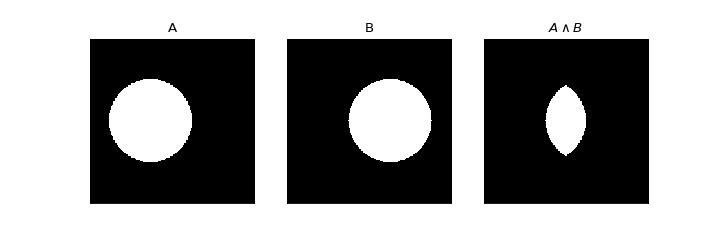
\includegraphics[width=\textwidth]{ocv_AND}
    \caption{AND}
    \label{fig:ocv_and}
\end{figure}
\end{ex}

\subsubsection{Logical OR}

The OR operator takes in two images and determines the values of the third images pixels based on the following truth table:

\begin{table}[H]
    \centering
    \def\arraystretch{1.1}%
    \begin{tabular}{ c c c } 
	\hline
	A & B & Q \\
	\hline
	0 & 0 & 0 \\
	0 & 1 & 1 \\
	1 & 0 & 1 \\
	1 & 1 & 1 \\
	\hline
    \end{tabular}
\end{table}

\noindent Mathematically it is defined as:

\begin{equation}
    Q(i,j) = P_1(i, j) \lor P_2(i, j) 
\end{equation}

\func{np.logical_or(x1, x2)}{Computes the truth value of x1 OR x2 element-wise.}

\begin{ex}OR
\begin{lstlisting}[language=Python]
np.logical_or(circle_r, circle_l)
\end{lstlisting}
\begin{figure}[H]
    \centering
    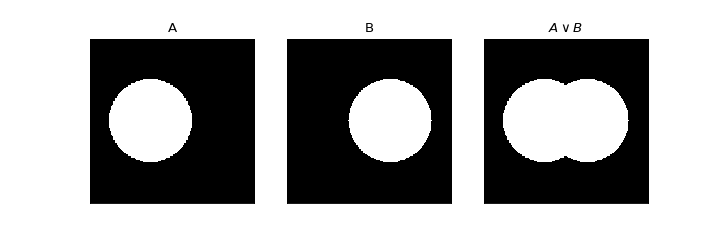
\includegraphics[width=\textwidth]{ocv_OR}
    \caption{OR}
    \label{fig:ocv_or}
\end{figure}
\end{ex}

\begin{rem}
    The OR operator can be used to computed the union of images, hence highlighting all pixels that are in the first or second image.
\end{rem}


\subsubsection{Logical XOR}


The exclusive or (XOR) operator takes in two images and determines the values of the third images pixels based on the following truth table:

\begin{table}[H]
    \centering
    \def\arraystretch{1.1}%
    \begin{tabular}{ c c c } 
	\hline
	A & B & Q \\
	\hline
	0 & 0 & 0 \\
	0 & 1 & 1 \\
	1 & 0 & 1 \\
	1 & 1 & 0 \\
	\hline
    \end{tabular}
\end{table}

\noindent Mathematically it is defined as:

\begin{equation}
    Q(i,j) = P_1(i, j) \veebar P_2(i, j) 
\end{equation}

\func{np.logical_xor(x1, x2)}{Computes the truth value of x1 XOR x2 element-wise.}

\begin{ex}XOR
\begin{lstlisting}[language=Python]
np.logical_xor(circle_r, circle_l)
\end{lstlisting}
\begin{figure}[H]
    \centering
    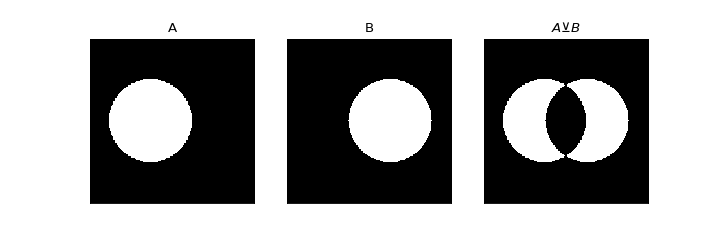
\includegraphics[width=\textwidth]{ocv_XOR}
    \caption{XOR}
    \label{fig:ocv_xor}
\end{figure}
\end{ex}

\begin{rem}
XOR can be used to detect changes in images, since pixels which did not change in an image are removed.
\end{rem}

\subsubsection{Logical NOT}

The NOT operator takes in an image and determines the values of the output image pixels based on the following truth table:

\begin{table}[H]
    \centering
    \def\arraystretch{1.1}%
    \begin{tabular}{ c c } 
	\hline
	A & Q \\
	\hline
	1 & 0 \\
	0 & 1 \\
	\hline
    \end{tabular}
\end{table}

\noindent Mathematically it is defined as:

\begin{equation}
    Q(i,j) = \neg P_1(i, j) 
\end{equation}

\func{np.logical_not(x)}{Computes the truth value of NOT x}

\begin{ex}NOT
\begin{lstlisting}[language=Python]
np.logical_not(circle)
\end{lstlisting}
\begin{figure}[H]
    \centering
    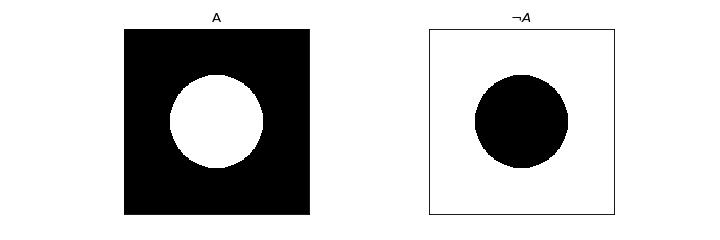
\includegraphics[width=\textwidth]{ocv_NOT}
    \caption{NOT}
    \label{fig:ocv_NOT}
\end{figure}
\end{ex}


\break


\subsection{Image Thresholding}

\subsubsection{Simple Thresholding}

Thresholding provides a straightforward way to perform image segmentation. For instance in many applications it is necessary to separate objects of interest, from the background regions of an image. It is also useful to see what regions of an image consist of pixels whose values are in a specific range.

The simplest way to apply thresholding is to set every pixel above a certain limit $ T $ to the maximum value $ M $ and those below to 0.

\begin{equation}
    s =\begin{cases}
    M, & \text{if $ r > T$}.\\
    0, & otherwise.
  \end{cases}
\end{equation}\\

\func{cv.threshold(src, thresh, maxValue, type)}{Applies a fixed-level threshold to each array element.}

\begin{ex} Basic Thresholding
\begin{lstlisting}[language=Python]
thresh = 160
img = cv.imread("./range.png")
arr, res1 = cv.threshold(img, thresh, 255, type=cv.THRESH_BINARY) 
arr, res2 = cv.threshold(img, thresh, 255, type=cv.THRESH_BINARY_INV) 
arr, res3 = cv.threshold(img, thresh, 255, type=cv.THRESH_TRUNC) 
arr, res4 = cv.threshold(img, thresh, 255, type=cv.THRESH_TOZERO) 
arr, res5 = cv.threshold(img, thresh, 255, type=cv.THRESH_TOZERO_INV) 
\end{lstlisting}
\begin{figure}[h!]
    \centering
    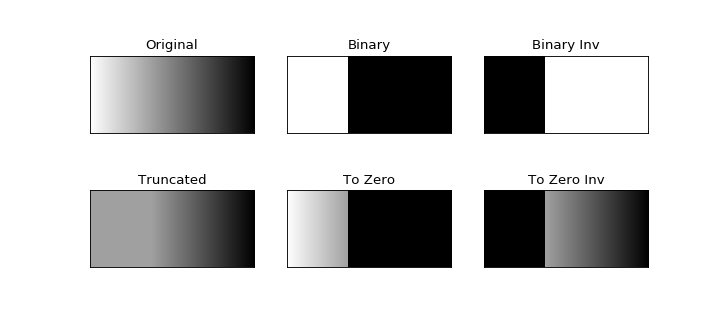
\includegraphics[width=\textwidth]{ocv_ith_basic}
    \caption{Basic Thresholding}
    \label{fig:ocv_ith_bas}
\end{figure}
\end{ex}

The available thresholds in OpenCV are:

\begin{table}[h!]
    \centering
    \def\arraystretch{1.1}%
    \begin{tabular}{ p{5cm} p{7cm} } 
	\hline
	Enumerator & Description \\
	\hline
	\textbf{\footnotesize{THRESH\_BINARY}} & 
	\begin{equation*}
	    s =\begin{cases}
		M, & \text{if $ r > T$}.\\
		0, & otherwise.
	    \end{cases}
	\end{equation*}\\

	\textbf{\footnotesize{THRESH\_BINARY\_INV}} & 
	\begin{equation*}
	    s =\begin{cases}
		0, & \text{if $ r > T$}.\\
		M, & otherwise.
	    \end{cases}
	\end{equation*}\\

	\textbf{\footnotesize{THRESH\_TRUNC}} & 
	\begin{equation*}
	    s =\begin{cases}
		M, & \text{if $ r > T$}.\\
		r, & otherwise.
	    \end{cases}
	\end{equation*}\\

	\textbf{\footnotesize{THRESH\_TOZERO}} & 
	\begin{equation*}
	    s =\begin{cases}
		r, & \text{if $ r > T$}.\\
		0, & otherwise.
	    \end{cases}
	\end{equation*}\\

	\textbf{\footnotesize{THRESH\_TOZERO\_INV}} & 
	\begin{equation*}
	    s =\begin{cases}
		0, & \text{if $ r > T$}.\\
		r, & otherwise.
	    \end{cases}
	\end{equation*}\\

	\textbf{\footnotesize{THRESH\_OTSU}} & Use Otsu algorithm to choose the optimal threshold value. \\

	\textbf{\footnotesize{THRESH\_TRIANGLE}} & Use Triangle algorithm to choose the optimal threshold value. \\
	\hline
    \end{tabular}
    \caption{Structuring Elements}
    \label{table:col_struct_el}
\end{table}

\subsubsection{Adaptive Thresholding}

Adaptive thresholding takes a grayscale image and outputs a binary image representing the segmentation. For each pixel a threshold is calculated. The threshold is then used to determine if the value of the pixel is set to the maximum or 0.\\

There are two methods available in OpenCV: mean thresholding and Gaussian thresholding. Both methods examine a local neighbourhood of pixels in order to determine the optimal threshold value.\\

\begin{rem}
The size of the neighbourhood has be to sufficiently large enough to cover both foreground and background pixels.\\
\end{rem}


\func{cv.adaptiveThreshold(src, maxVal, adaptiveMethod, thresholdType, size, C)}{Applies a threshold to an array, the constant C is subtracted from the mean / weighted mean.}


\begin{ex} Adaptive Thresholding
\begin{lstlisting}[language=Python]
img = cv.imread("./sudoku.png", 0)
img = cv.medianBlur(img, 5)

res_mean = cv.adaptiveThreshold(img, 255, cv.ADAPTIVE_THRESH_MEAN_C, cv.THRESH_BINARY, 11, 2)
res_gaus = cv.adaptiveThreshold(img, 255, cv.ADAPTIVE_THRESH_GAUSSIAN_C, cv.THRESH_BINARY, 11, 2) 
\end{lstlisting}
\begin{figure}[h!]
    \centering
    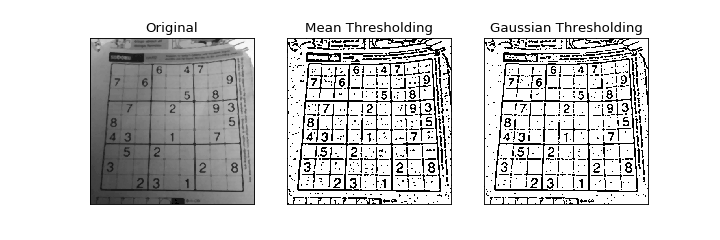
\includegraphics[width=\textwidth]{ocv_ith_adaptive}
    \caption{Adaptive Thresholding}
    \label{fig:ocv_ith_adap}
\end{figure}
\end{ex}


\subsubsection{Otsu's Binarization}

Otsu binarization is used to automatically determine an optimal threshold $ t $  based on the distribution of pixel intensity. For instance consider a bimodal image (an image with two intensity peaks), a good threshold would exist somewhere between the two peaks. Otsu's method determines the optimal value by separating the two regions such that the weighted within-class variance is minimized, \textit{i.e.}:

\begin{equation}
    \sigma_w^2(t) = q_1(t)\sigma_1^2(t) + q_2(t)\sigma_2^2(t)
\end{equation}
\noindent Where:
\begin{gather*}
    q_1(t) = \sum_{i=1}^{t} P(i) \qquad q_2(t) = \sum_{i=t+1}^{I} P(i) \\
    \mu_1(t) = \sum_{i=1}^{t} \frac{iP(i)}{q_1(t)} \qquad \mu_2(t) = \sum_{i=t+1}^{I} \frac{iP(i)}{q_2(t)} \\
    \sigma_1^2(t) = \sum_{i=1}^{t} [i-\mu_1(t)]^2 \frac{P(i)}{q_1(t)} \qquad  \sigma_2^2(t) = \sum_{i=t+1}^{I} [i-\mu_2(t)]^2 \frac{P(i)}{q_2(t)}
\end{gather*}


In order to apply Otsu Binarization in OpenCV the \lstinline{threshold} function is used.


\begin{ex} Otsu Binarization
\begin{lstlisting}[language=Python]
img = cv.imread("./noisy.png", 0)
img = cv.GaussianBlur(img, (5, 5), 0)

thresh, bin_img = cv.threshold(img, 0, 255, cv.THRESH_BINARY + cv.THRESH_OTSU) 
\end{lstlisting}
\begin{figure}[h!]
    \centering
    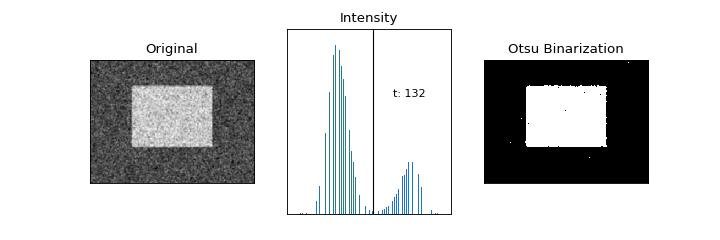
\includegraphics[width=\textwidth]{ocv_otsu}
    \caption{Otsu Binarization applied to a noisy image}
    \label{fig:ocv_otsu}
\end{figure}

\begin{rem}
A line has been added to the histogram to show that the optimal threshold $ t = 132 $.
\end{rem}
\end{ex}



\break


\subsection{Image Smoothing}


\subsubsection{A note on Convolution}

\begin{df}Convolution

A mathematical operation denoted by $ * $ applied on two functions $ f, g $ that expresses how the shape of $ f $ is modified by $ g $.

\end{df}

\noindent For continuous functions it is defined as:

\begin{equation}
    (f * g)(t) \triangleq \int_{-\infty}^{\infty} f(\tau)g(t - \tau) d\tau
\end{equation}

\noindent For discrete functions it is defined as:

\begin{equation}
    (f * g)[n] = \sum_{m=-\infty}^{\infty}f[m]g[n -m]
\end{equation}

\noindent Some properties of convolution include:\\
\begin{description}
    \item Commutativity $ f * g = g * f $

    \item Associativity $ f * (g * h) = (f * g) * h $

    \item Distributivity $ f * (g + h) = (f * g) + (f * h) $

    \item Multiplicative Identity $ f * \delta = f $
\end{description}

\hfill

\noindent In image processing convolution provides a means of combining two arrays generally of different sizes but of the same dimensionality; to produce a third array.

\begin{ex} Input and Kernel Arrays\\

\noindent Consider and Image $ \pmb{I} $

\begin{equation*}
    \begin{bmatrix}
    I_{1, 1} & I_{1, 2} & \dots & I_{1, n-1} & I_{1, n} \\
    I_{2, 1} & I_{2, 2} & \dots & I_{2, n-1} & I_{2, n} \\
    \vdots & \vdots & \ddots & \vdots & \vdots \\ 
    I_{m-1, 1} & I_{m-1, 2} & \dots & I_{m-1, n-1} & I_{m-1, n} \\
    I_{m, 1} & I_{m, 2} & \dots & I_{m, n-1} & I_{m, n} \\
    \end{bmatrix}
\end{equation*}

\hfill

\noindent And Kernel $ \pmb{K} $

\begin{equation*}
    \begin{bmatrix}
	K_{1,1} & K_{1,2} & K_{1,3} \\
	K_{2,1} & K_{2,2} & K_{2,3} \\
    \end{bmatrix}
\end{equation*}

\hfill

\noindent The convolution is performed by sliding the Kernel $ \pmb{K} $ over the Image $ \pmb{I} $, such that all the positions fit $ \pmb{K} $ entirely. Each position corresponds to a single output value for example:

\begin{equation*}
    O_{5, 7} = I_{5, 7}K_{1,1} + I_{5, 8}K_{1,2} + I_{5, 9}K_{1,3} + I_{6, 7}K_{2,1} + I_{6, 8}K_{2,2} + I_{6, 9}K_{2,3}
\end{equation*}

\hfill

\noindent Or more generally:\\
\begin{equation}
O(i,j) = \sum_{k=1}^{m}\sum_{l=1}^{n}I(i + k - 1, j + l - 1)K(k, l)
\end{equation}

\end{ex}

\begin{nb}
    Many implementations of convolution relax the constraint that the kernel can only be moved into places where it fits entirely; producing a larger output image due to the borders.
\end{nb}

\begin{rem}
    Convolution can be used to implement many different operators, in particular: spatial filters, feature detectors, image smoothing, edge detectors and so forth.
\end{rem}

\subsubsection{Image Smoothing Theory}

Smoothing is a simple and frequently used image processing operation. It is commonly used to reduce noise and produce a less pixelated image. The most basic smoothing operation is linear smoothing. Smoothing operations are typically defined as:


\begin{equation}
    g(i, j) = \sum_{k, l} f(i + k, j + l) h(k, l)
\end{equation}

\noindent Where:\\
\begin{description}
    \item $ g(i, j) $ pixel value\\
    \item $ f(i + k,j + l) $ input pixel values\\
    \item $ h(k, l) $ kernel\\
\end{description}

\begin{rem}
The kernel is just a matrix of coefficients.
\end{rem}

\subsubsection{Normalized Box or Mean Filter}

Normalized box or mean filtering is a simple filter, where each output pixel is the mean of its kernel neighbours, each neighbour's value contributes with equal weight to the value of the output pixel $ O $.

\begin{equation}
    K = \frac{1}{K_{width} \cdot K_{height}}
    \begin{bmatrix}
	1 & \dots & 1 \\
	\vdots & \ddots & \vdots \\ 
	1 & \dots & 1
    \end{bmatrix}
\end{equation}

\begin{ex}$ 3 \times 3 $ Mean Filter

    \noindent Consider the Kernel $ \pmb{K} $
\begin{equation*}
    \frac{1}{9}\begin{bmatrix}
	1 & 1 & 1 \\
	1 & 1 & 1 \\
	1 & 1 & 1
    \end{bmatrix}
\end{equation*}

\noindent And a region of an Image $ \pmb{I} $\\

\begin{equation*}
\begin{matrix}
    \cdot & \pmb{1} & \pmb{2}  & \pmb{3} \\
    \pmb{1} & 123 & 125 & 126 \\ 
    \pmb{2} & 122 & 124 & 126 \\
    \pmb{3} & 118 & 120 & 150 
\end{matrix}
\end{equation*}

\noindent The value of the pixel at $ 2, 2\ \pmb{p} $ is given by:
\begin{align*}
    O_{2,2} = &\ \frac{1}{9}(123 + 122 + 118 + 125 + 124 + 120 + 126 + 126 + 150) \\
	    = &\ 126
\end{align*}
\end{ex}

\begin{rem}
    A Mean filter provides a simple way to smooth an image, however this also provides the non-desirable effect of smoothing edges.
\end{rem}

\subsubsection{Median Filtering}

Median filtering considers each pixel of the image in turn and looks at its nearby neighbours to determine whether or not its representative of the surroundings. 

\begin{ex} Median Filtering
\begin{equation}
    \begin{matrix}
	\cdot & .  & . & .  & . & . & \cdot \\
	\cdot & 123 & 125  & 126  & 130  & 140 & \cdot \\
	\cdot & 122 & \pmb{124} & \pmb{126} & \pmb{127} & 135 & \cdot \\
	\cdot & 118 & \pmb{120} & \pmb{150} & \pmb{125} & 134 & \cdot \\
	\cdot & 119 & \pmb{115} & \pmb{119} & \pmb{123} & 133 & \cdot \\
	\cdot & 111 & 116  & 110  & 120  & 130 & \cdot \\
	\cdot & ^.  & ^. & ^.  & ^. & ^. & \cdot\\
    \end{matrix} \rightarrow \text{median value: 124} 
\end{equation}

The central point $ 150 $ is unrepresentative of the surrounding pixels: $ 115, 119, 120,\\ 123, 124, 125, 126, 127, 150 $ and so it is replaced with a value of $ 124 $. 
\end{ex}

\begin{nb}
In the above example a $ 3 \times 3 $ neighbourhood is used; larger neighbourhoods will produce more severe smoothing.\\
\end{nb}

\begin{rem}
    In practise median filtering does a better job than mean (box) filtering in terms of preserving detail in an image.\\
\end{rem}

\begin{rem}
Median filters are also much better at preserving sharp edges as they do not generate entirely new pixel values but use values already present in the image.\\
\end{rem}

\subsubsection{Gaussian Filter}

Gaussian Filtering or Gaussian Blur Filtering is amongst one of the more useful filters, however is more computationally intense (and therefore slower). Gaussian filtering provides greater weight to the pixels closest to the output pixel, and decreases the weight as the spatial distance of the pixels increases. 

\begin{equation}
    G_{\sigma}(x, y) = \frac{1}{2\pi\sigma^2}e^{-\frac{x^2 + y^2}{2 \sigma^2}}
\end{equation}

\noindent Which produces the following distribution

\begin{figure}[h!]
    \centering
    
\includegraphics[width=0.6\textwidth]{plot_2dnorm}
    \caption{2D Gaussian Distribution}
    \label{fig:2d_norm}
\end{figure}

\begin{rem}
The idea behind Gaussian smoothing is to use the 2D distribution as a point-spread function, i.e. produce a discrete approximation to the Gaussian function s.t. we can perform the convolution. In reality the 2D Gaussian Distribution is infinitely large; which would produce a kernel that is infinitely large as such an approximation is needed.
\end{rem}

\noindent The 2D Gaussian Kernel is given by:
\begin{equation}
    G_{\sigma}(x) = \frac{1}{2\pi\sigma^2}e^{-\frac{x^2}{2 \sigma^2}}
\end{equation}

\hfill

\noindent The Gaussian Blur Filtered Image is defined as:
\begin{equation}
    GB[I]_p = \sum_{q \in \mathcal{S}} G_{\sigma}(|\pmb{p} - \pmb{q}|)I_q
\end{equation}

\begin{ex} Gaussian Kernel $ \sigma = 1.0 $, 
\begin{equation*}
    G_{1} = \frac{1}{273}\begin{bmatrix}
	1 & 4  & 7  & 4  & 1 \\
	4 & 16 & 26 & 16 & 1 \\
	7 & 26 & 41 & 26 & 1 \\
	4 & 16 & 26 & 16 & 1 \\
	1 & 4  & 7  & 4  & 1
    \end{bmatrix}
\end{equation*}
\end{ex}

\noindent Once a suitable kernel is calculated then the Gaussian smoothing can be performed.

\begin{rem}
    Given that the Kernel is circularly symmetric the convolution can be done with 1D matrices first in the $ x $ direction and then in the $ y $ 
\end{rem}


\subsubsection{Bilateral Filtering}

Bilateral filtering is a simple, non-iterative scheme of edge-preserving smoothing.

\begin{rem}
    Bilateral Filtering was discovered in 1995 and used in 1997 as part of the SUSAN framework. Since then it has grown in popularity and is widely adopted in image processing applications \cite{bilateral_filtering}
\end{rem}

\hfill

\noindent Formally Bilateral Filtering is given by:

\begin{equation}
    BF(I)_p = \frac{1}{W_p}\sum_{q \in S}G_{\sigma_s}(|\pmb{p} - \pmb{q}|) G_{\sigma_\tau}(I_p - I_q)I_q
\end{equation}

\noindent Where $ W_p $ is a normalization factor:

\begin{equation}
    W_p = \sum_{q \in S}G_{\sigma_s}(|\pmb{p} - \pmb{q}|) G_{\sigma_\tau}(I_p - I_q)
\end{equation}

\hfill

\noindent Bilateral Filtering has several qualities:
\begin{itemize}
    \item intuitive, pixels are replaced by an average of their neighbours.

    \item dependant on two parameters, size and contrast.
    
    \item Non-iterative, parameter effect is not cumulative.
\end{itemize}

Typically it is assumed that spatial variation occurs slowly in images so it is appropriate for nearer pixels to have similar values. Simple filters such as Normalized Box do not account for the increased spacial variance that occurs at edges and tends to blur them. Bilateral Filtering is a solution that smooths out regions and prevents averaging of pixel values around edges.\\


\begin{ex} Intuition behind Bilateral Filtering\\

\noindent Consider:
\begin{equation*}
G_{\sigma_s}(|\pmb{p} - \pmb{q}|)I_q
\end{equation*}

\noindent This is the definition for the Gaussian Blur Filter.\\

\noindent Hence the main component behind BF is:
\begin{equation*}
    G_{\sigma_\tau}(I_p - I_q)
\end{equation*}

\noindent The effect is controlled by $ \sigma_\tau $. For instance larger values of $ \sigma_\tau $ will smooth pixels over larger ranges of contrast.
\end{ex}

\begin{figure}[h!]
    \centering
    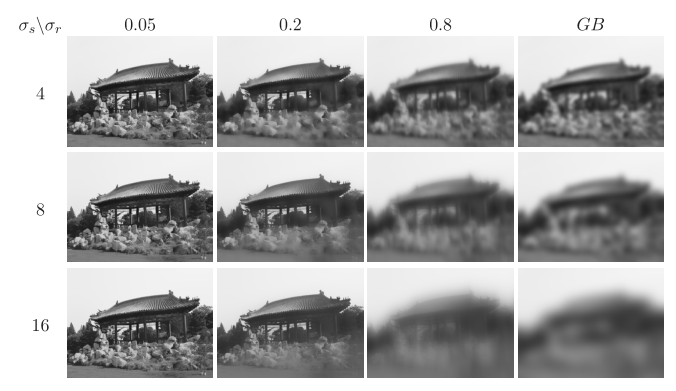
\includegraphics[width=\textwidth]{bilat_filt_coeffs}
    \caption{Bilateral Filtering Coefficients}
    \label{fig:bilat_filt}
\end{figure}

\begin{nb}
The GB column represents the image under a Gaussian Blur Filter with parameter $ \sigma_s $
\end{nb}


\begin{figure}[h!]
    \centering
    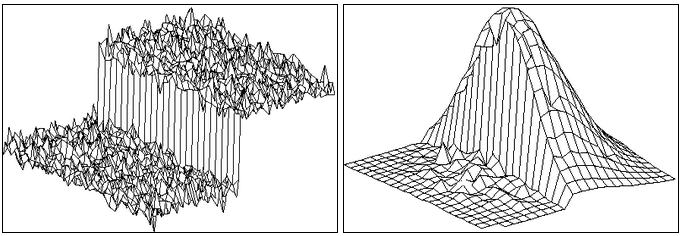
\includegraphics[width=\textwidth]{bilat_filt_effect}
    \caption{Bilateral Filtering}
    \label{fig:bilat_filt_alt}
\end{figure}

The effect of Bilateral Filtering is demonstrated above, where both regions of the image have been smoothed and the contrast / edge is preserved in the image.


\break


\subsubsection{Smoothing Functions in OpenCV}

\func{cv.blur(src, dst, ksize, anchor=(-1, -1), borderType=BORDER_DEFAULT)}{
Blurs an image using a normalized box filter.
}

\begin{ex} Mean Filtering
\begin{lstlisting}[language=Python]
lena = cv.imread("./lena.png")
lena_1 = cv.blur(lena, (10,10))
lena_2 = cv.blur(lena, (30, 30))
\end{lstlisting}
\begin{figure}[h!]
    \centering
    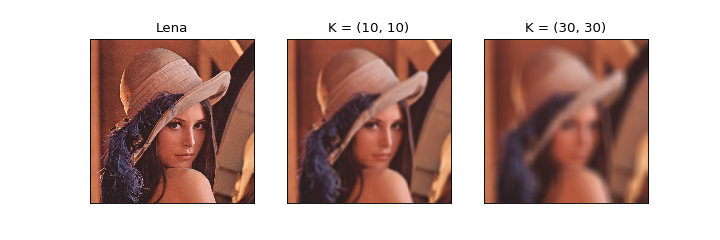
\includegraphics[width=\textwidth]{ocv_mean_filtering}
    \caption{Mean Filtering}
    \label{fig:ocv_mean_filt}
\end{figure}
\end{ex}

\func{cv.medianBlur(src, dst, ksize)}{
Blurs an image using the median filter. ksize must be an odd number greater than 1, \textit{ex:} 3, 5, 7}

\begin{ex} Median Filtering
\begin{lstlisting}[language=Python]
lena_1 = cv.medianBlur(lena, 9)
lena_2 = cv.medianBlur(lena, 91)
\end{lstlisting}
\begin{figure}[h!]
    \centering
    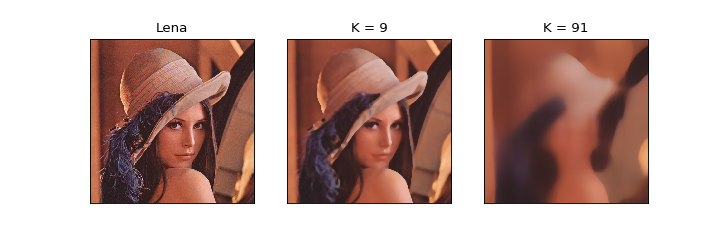
\includegraphics[width=\textwidth]{ocv_median_filtering}
    \caption{Median Filtering
    }
    \label{fig:ocv_median_filt}
\end{figure}
\end{ex}


\break


\func{cv.GaussianBlur(src, dst, ksize, sigmaX, sigmaY=0)}{Blurs an image using a Gaussian filter.}

\begin{ex} Gaussian Filtering
\begin{lstlisting}[language=Python]
lena_1 = cv.GaussianBlur(lena, (9, 9), 1)
lena_2 = cv.GaussianBlur(lena, (31, 31), 5)
\end{lstlisting}
\begin{figure}[h!]
    \centering
    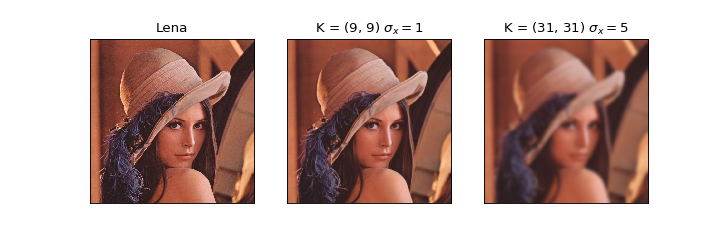
\includegraphics[width=\textwidth]{ocv_gaussian_filtering}
    \caption{Gaussian Filtering}
    \label{fig:ocv_gauss_filt}
\end{figure}
\end{ex}

\func{cv.bilateralFilter(src, dst, d, sigmaColor, sigmaSpace)}{Applies the bilateral filter to an image, for simplicity sigma values can be the same, large sigma values $ > 150 $ will have a strong effect, giving a cartoonish look. Filter size $ d > 5 $, are slow. $ d = 5 $ is recommended, $ d= 9$ is fine for offline applications.
}

\begin{ex}Bilateral Filtering
\begin{lstlisting}[language=Python]
lena_1 = cv.bilateralFilter(lena, 5, 75, 75)
lena_2 = cv.bilateralFilter(lena, 19, 400, 30)
\end{lstlisting}
\begin{figure}[h!]
    \centering
    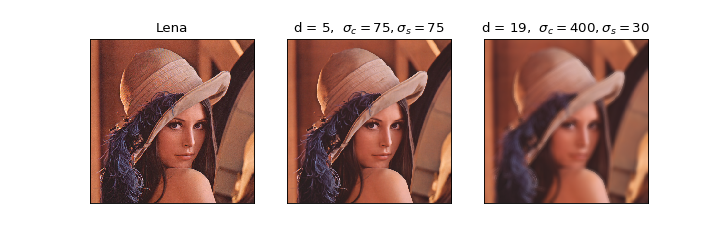
\includegraphics[width=\textwidth]{ocv_bilateral_filtering}
    \caption{Bilateral Filtering}
    \label{fig:ocv_bilat_filt}
\end{figure}
\end{ex}


\break


\section{OpenCV: Image Processing - Transformations}


\subsection{Geometric Transformations}

\subsubsection{Scaling}

Scaling compresses or expands an image along the coordinate directions.\\


\noindent An image or region of pixels can be compressed by sub sampling, this method is computationally simple, for instance a random pixel can be selected from a neighbourhood or an interpolation of pixel values can be used.

\begin{ex} Compression
\begin{gather*}
    I = \begin{matrix}
	2 & 2 & 2 & 2 \\
	6 & 6 & 6 & 6 \\
	2 & 2 & 2 & 2 \\
	6 & 6 & 6 & 6 \\
    \end{matrix}  \\
    \text{Single Pixel Selection} \qquad  \qquad
\text{Interpolation} \\
    \begin{matrix}
	2 & 2  \\
	2 & 2  \\
    \end{matrix} \qquad \qquad \qquad \qquad \quad
    \begin{matrix}
	4 & 4  \\
	4 & 4  \\
    \end{matrix} 
\end{gather*}
\end{ex}

\begin{rem}
    When a single pixel is selected (potentially at random) it is used to represent the compressed region. However a linear (or other functional) interpolation can provide a better representation of the image.
\end{rem}


\noindent Similarly when an image zoomed it can be done through pixel replication or interpolation.

\begin{ex} Zooming
\begin{gather*}
    I = \begin{matrix}
	2 & 5 \\
	2 & 5 \\
    \end{matrix} \\
    \text{Replication} 
    \qquad \qquad \qquad \qquad
    \text{Interpolation} \\
    \begin{matrix}
	2 & 2 & 5 & 5 \\
	2 & 2 & 5 & 5 \\
	2 & 2 & 5 & 5 \\
	2 & 2 & 5 & 5 \\
    \end{matrix} 
    \qquad \qquad \qquad \qquad \quad
    \begin{matrix}
	2 & 3 & 4 & 5 \\
	2 & 3 & 4 & 5 \\
	2 & 3 & 4 & 5 \\
	2 & 3 & 4 & 5 \\
    \end{matrix} 
\end{gather*}
\end{ex}

\noindent Image scaling in OpenCV is done with the \lstinline{resize} function.\\

\func{cv.resize(src, dsize, fx, fy, interpolation=INTER_LINEAR)}{Resizes an image down or up to the specified size}

\begin{ex} Resizing
\begin{lstlisting}[language=Python]
img = cv.imread("./lena.png")
res = cv.resize(img, None, fx=2, fy=2)
# height, width = img.shape[:2]
# res = cv.resize(img, (1*width, 2*height))
\end{lstlisting}

\begin{nb}
    \lstinline{dsize} is a tuple specifying an exact width and height to resize to.
\end{nb}
\end{ex}


\begin{table}[H]
    \centering
    \def\arraystretch{1.1}%
    \begin{tabular}{ p{5cm} p{7cm} } 
	\hline
	Enumerator & Description \\
	\hline
	\textbf{\footnotesize{INTER\_NEAREST}} & nearest neighbor interpolation \\

	\textbf{\footnotesize{INTER\_LINEAR}} & bilinear interpolation \\

	\textbf{\footnotesize{INTER\_CUBIC}} & bicubic interpolation \\

	\textbf{\footnotesize{INTER\_AREA}} & resampling using pixel area relation. It may be a preferred method for image decimation, as it gives moir\'e-free results.\\

	\textbf{\footnotesize{INTER\_LANCZOS4}} & Lanczos interpolation over $ 8 \times 8 $ neighbourhood \\

	\textbf{\footnotesize{INTER\_LINEAR\_EXACT}} & Bit exact bilinear interpolation \\

	\textbf{\footnotesize{INTER\_MAX}} & mask for interpolation codes \\

	\textbf{\footnotesize{WARP\_FILL\_OUTLIERS}} & Fills all of the destination image pixels. If some of them correspond to outliers in the source image, they are set to zero \\

	\hline
    \end{tabular}
    \caption{Interpolation Flags}
\end{table}


\subsubsection{Rotation}

Rotation is most commonly used to improve the visual appearance of an image. The operation is performed by geometric transformation which maps the input position $ (x_1, y_1) $ to the output position $ (x', y') $ via a rotation about an origin $ O $ over a given angle $ \theta $.\\

\noindent In OpenCV the new pixel positions $ (x', y') $ are determined using the matrix $ \pmb{M} $:

\begin{equation}
    \pmb{M} = \begin{bmatrix}
	\alpha & \beta & (1-\alpha)x_0 - \beta y_0 \\
       -\beta & \alpha & (1-\alpha)y_0 + \beta x_0 \\
	0 & 0 & 1
    \end{bmatrix} 
\end{equation} 

\noindent Where:
\begin{gather*}
    \alpha = scale \cdot \cos(\theta) \\
    \beta = scale \cdot \sin(\theta) \\
    x_0, y_0:\ \text{origin}
\end{gather*} \\

\noindent $ (x', y') $ are given by:

\begin{equation*}
    \begin{bmatrix}
	x' \\
	y' \\
	1
    \end{bmatrix} =  
    \pmb{M}
    \begin{bmatrix}
	x_1 \\
	y_1 \\
	1
    \end{bmatrix}
\end{equation*} \\

The rotation matrix $ \pmb{M} $ is determined by the \lstinline{getRotationMatrix2D} function, and the rotation carried out by \lstinline{warpAffine}.\\

\func{cv.getRotationMatrix2D(center, angle, scale)}{Calculates an affine matrix of 2D rotation.} \\

\func{cv.warpAffine(src, M, dsize, flags=INTER_LINEAR)}{Applies an affine transformation to an image. }

\begin{ex} Rotation
\begin{lstlisting}[language=Python]
rows, cols = img.shape
center = ((cols - 1)/2.0, (rows - 1)/2.0)
M = cv.getRotationMatrix2D(center, 45, 1)
res = cv.warpAffine(img, M, (cols, rows))
\end{lstlisting}

\begin{figure}[h!]
    \centering
    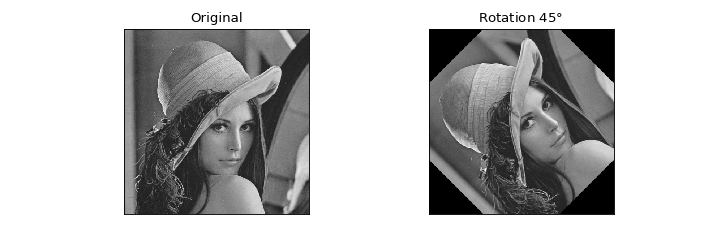
\includegraphics[width=\textwidth]{ocv_gt_rotation}
    \caption{Rotation}
    \label{fig:ocv_gt_rot}
\end{figure}
\end{ex}

\subsubsection{Translation}

Translation is often used to improve visual appearance. It also has a role as a preprocessor in applications where two or more images are involved. Translation maps each pixel in an input image $ (x_1, y_1) $ to a new position in an output image $ (x', y') $. The dimensionality of the two images is often (but not strictly) the same. 

\begin{nb}
Translation is a special case of affine transformation.
\end{nb}

\noindent Translation is performed with the affine matrix $ \pmb{M} $ given by:

\begin{equation}M =
    \begin{bmatrix}
	1 & 0 & t_x \\
	0 & 1 & t_y
    \end{bmatrix}
\end{equation}

\noindent Hence $ (x', y') $ is determined by:

\begin{equation*}
    \begin{bmatrix}
	x' \\
	y' \\
	1
    \end{bmatrix} =  
    \pmb{M}
    \begin{bmatrix}
	x_1 \\
	y_1 \\
	1
    \end{bmatrix}
\end{equation*} \\

\begin{ex} Translation
\begin{lstlisting}[language=Python]
M =np.float32([
    [1, 0, 100],
    [0, 1, 100]
])
res = cv.warpAffine(img, M, img.shape)
\end{lstlisting}
\begin{figure}[h!]
    \centering
    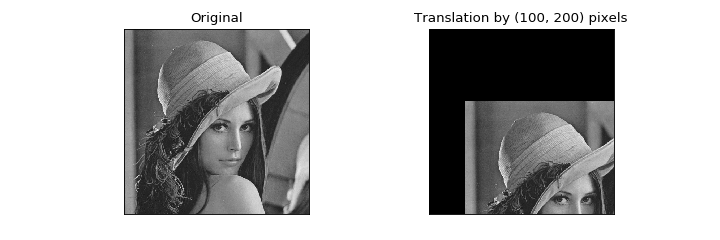
\includegraphics[width=\textwidth]{ocv_gt_translation}
    \caption{Translation}
    \label{fig:ocv_gt_trans}
\end{figure}
\end{ex}


\subsubsection{Affine Transformation}

Occasionally geometric distortion can be introduced to an image due to perspective irregularities. Perspective irregularities typically occur due to the position of the camera with respect to the scene; altering the apparent dimensions of the scene geometry. Applying an affine transformation to a uniformly distorted image can correct the distortion. \\

\noindent Affine transformation is commonly written as:
\begin{equation}
    \begin{bmatrix}
	x' \\
	y'
    \end{bmatrix} =  
    \pmb{A}
    \begin{bmatrix}
	x_1 \\
	y_1 \\
    \end{bmatrix}
    + 
    \pmb{B}
\end{equation}

\noindent Affine matrices can be used to carry out different geometric operations as shown previously.

\begin{ex} Affine transformation matrices and Geometric operations\\

\noindent Scaling \\
\begin{equation*}
    \pmb{A} =
    \begin{bmatrix}
	a_{11} & 0 \\
	0 & a_{22} \\
    \end{bmatrix}
    ,\ 
    \pmb{B} = 
    \begin{bmatrix}
	0 \\
	0 \\
    \end{bmatrix}
\end{equation*} \\

\noindent Rotation \\
\begin{equation*}
    \pmb{A} =
    \begin{bmatrix}
	\cos(\theta) & -\sin(\theta) \\
	\sin(\theta) & \cos(\theta) \\
    \end{bmatrix}
    ,\
    \pmb{B} = 
    \begin{bmatrix}
	0 \\
	0 \\
    \end{bmatrix}
\end{equation*} \\

\noindent Translation \\
\begin{equation*}
    \pmb{A} =
    \begin{bmatrix}
	1 & 0 \\
	0 & 1 \\
    \end{bmatrix}
    ,\ 
    \pmb{B} = 
    \begin{bmatrix}
	t_x \\
	t_y \\
    \end{bmatrix}
\end{equation*}\\

\noindent In order to calculate the affine matrix in OpenCV \lstinline{getAffineTransform} is used.\\

\func{cv.getAffineTransform(src, dst)}{Calculates the affine transform from three pairs of corresponding points.}

\begin{ex} Affine Transformation
\begin{lstlisting}[language=Python]
pts1 = np.float32([ 
    [20, 20],
    [20, 100],
    [100, 20]
])
pts2 = np.float32([ 
    [10, 50],
    [25, 110],
    [70, 60]
])
M = cv.getAffineTransform(pts1, pts2)
res = cv.warpAffine(img, M, (cols, rows))
\end{lstlisting}
\end{ex}
\begin{figure}[h!]
    \centering
    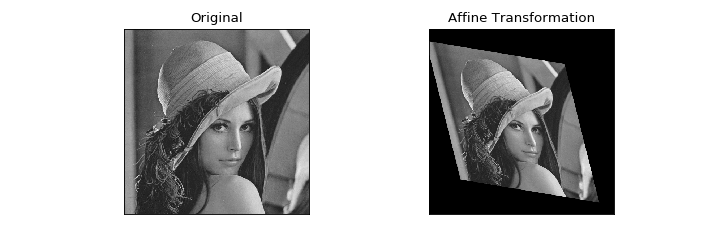
\includegraphics[width=\textwidth]{ocv_gt_afftran}
    \caption{Affine Transformation}
    \label{fig:ocv_gt_afftran}
\end{figure}
\end{ex}

\begin{rem}
Several different affine transformations can be combined to produce a resultant image. It is important to note that the order at which the operations occur is significant, for instance the effect of rotation followed by transformation may not be equivalent to the converse.
\end{rem}


\subsubsection{Perspective Transformation}

Perspective transformation uses a $ 3 \times 3 $ Matrix in order to map input points to the new points $ (x', y') $.\\

\func{cv.getPerspectiveTransform(src, dst, solveMethod=DECOMP_LU}{Calculates a perspective transform matrix from four pairs of corresponding points.}\\

\func{cv.warpPerspective(src, M, dsize, flags=INTER_LINEAR)}{Applies a perspective transformation to an image.}


\begin{ex} Perspective Transformation
\begin{lstlisting}[language=Python]
img = cv.imread("./sudoku.png")

pts1 = np.float32([[56, 65], [368, 52], [28, 387], [389, 390]])
pts2 = np.float32([[0, 0], [300, 0], [0, 300], [300, 300]])

M = cv.getPerspectiveTransform(pts1, pts2)
res = cv.warpPerspective(img,M,(300,300))
\end{lstlisting}
\begin{figure}[h!]
    \centering
    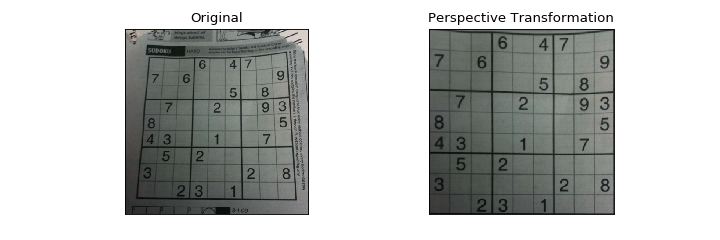
\includegraphics[width=\textwidth]{ocv_gt_pertran}
    \caption{Perspective Transformation}
    \label{fig:ocv_per_tran}
\end{figure}
\end{ex}

\begin{rem}
Among the four points chosen 3 should no be collinear.
\end{rem}


\break


\subsection{Morphological Transformations}

\subsubsection{Mathematical Morphology}

Mathematical morphology contributes a wide range of operators to image processing, all based around a few mathematical concepts from set theory. The operators are particularly useful for the analysis of binary images and common usages include edge detection, noise removal, image enhancement and image segmentation. 


The basic operations in morphology are erosion and dilation. Both operations require and image $ I $ and a kernel $ K $. For binary images, white pixels are taken as the foreground and black pixels denote the background. For grayscale images, the intensity represents the height above the base plane. 


Conceptually erosion and dilation work by translating the Kernel over various points in the input image and examining the intersection between the kernel coordinates and the input image coordinates. In the case of erosion the output image $ O $ consists of the points in which $ K $ can be translated while remaining within the input image.

\begin{rem}
    Other operators are defined as a combination of erosion and dilation along with set operators. \textit{ex.} opening, closing, skeletonization.
\end{rem}

\subsubsection{Erosion}

Erosion operators takes an image $ I $ and a Kernel $ K $ also referred to a structuring element. The structuring element determines the effect of the erosion on the input image. 

\begin{df} Erosion

The erosion of $ I $ by $ K $ is the set of all points $ x $ s.t. $ K_x \subseteq I $.

\begin{equation}
I \ominus K = \{ K_x \subseteq I \}
\end{equation}

\noindent Where:  

$ I $ is a set of Euclidean coordinates corresponding to the input binary image. 

$ K $ is the set of coordinates for the structuring element. 

$ K_x $ denotes the translation of $ K $ s.t. the origin is at $ x $

\end{df}

\begin{rem}
The mathematical definition for grayscale erosion is identical except the set of coordinates associated with the image are 3D instead of 2D. 
\end{rem}


\begin{ex} Erosion

\begin{equation*}
    I =\  \begin{matrix}
	& \vdots  & \vdots & \vdots  & \vdots & \vdots \\
	\dots & 1 & 1 & 1 & 1 & 1 & \dots \\
	\dots & 1 & 1 & 1 & 1 & 1 & \dots \\
	\dots & 1 & 1 & 1 & 1 & 1 & \dots \\
	\dots & 1 & 1 & \pmb{0} & 1 & 1 & \dots \\
	\dots & 1 & 1  & 1  & 1  & 1 & \dots \\
	& \vdots  & \vdots & \vdots  & \vdots & \vdots 
    \end{matrix}
\end{equation*}
\begin{equation*}
    K =\ \begin{bmatrix}
	1 & 1 & 1 \\
	1 & 1 & 1 \\
	1 & 1 & 1  
    \end{bmatrix}
\end{equation*}
For each pixel $ p $, $ K $ is superimposed over $ I $ if it`s fully contained then the value is retained else it is set to $ 0 $.\\

\noindent The erosion of $ I \text{ by } K $ is:
\begin{equation*}
    I \ominus K = \begin{matrix}
	& \vdots  & \vdots & \vdots  & \vdots & \vdots \\
	\dots & 1 & 1 & 1 & 1 & 1 & \dots \\
	\dots & 1 & 1 & 1 & 1 & 1 & \dots \\
	\dots & 1 & \pmb{0} & \pmb{0} & \pmb{0} & 1 & \dots \\
	\dots & 1 & \pmb{0} & \pmb{0} & \pmb{0} & 1 & \dots \\
	\dots & 1 & \pmb{0} & \pmb{0} & \pmb{0} & 1 & \dots \\
	& \vdots  & \vdots & \vdots  & \vdots & \vdots 
    \end{matrix}
\end{equation*}
\end{ex}

\begin{rem}
    In this case it is assumed that the origin of $ I $ is the centre.\\
\end{rem}

Grayscale erosion results in a decrease in intensity. Generally darkening the image. Bright regions are shrunk in size and dark regions grow. The effect is noticeable when there is a sharp increase in intensity. Regions with uniform intensity are left practically unchanged.

\begin{figure}[h!]
    \centering
    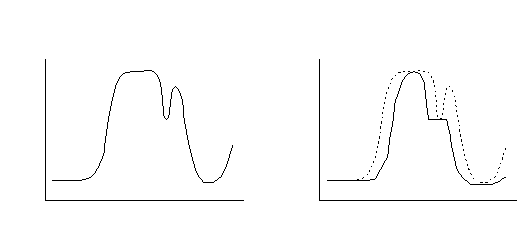
\includegraphics[width=\textwidth]{eroding}
    \caption{Grayscale erosion intensity change}
    \label{fig:eroding}
\end{figure}


\begin{nb}
    Eroding foreground pixels is the same as dilating background pixels. In other words Erosion is the \textit{dual} to dilation.
\end{nb}


\break


\subsubsection{Dilation}

Dilation is the second basic operator in the field of mathematical morphology. The basic effect is to gradually enlarge the boundaries of regions of foreground pixels. The dilation operator takes an input image $ I $ and a Kernel or structuring element $ K $. 


\begin{df} Dilation

The dilation of $ I $ by $ K $ is the set of all points $ x $ s.t. the intersect is non empty.

\begin{equation}
    I \oplus K = \{ K_x \cap I = \emptyset \}
\end{equation}

\noindent Where:  

$ I $ is a set of Euclidean coordinates corresponding to the input binary image. 

$ K $ is the set of coordinates for the structuring element. 

$ K_x $ denotes the translation of $ K $ s.t. the origin is at $ x $

\end{df}

\begin{ex} Dilation

\begin{equation*}
    I =\  \begin{matrix}
	& \vdots  & \vdots & \vdots  & \vdots & \vdots \\
	\dots & \pmb{0}  & 1 & 1 & 1 & 1 & \dots \\
	\dots & 1 & 1 & 1 & 1 & 1 & \dots \\
	\dots & 1 & 1 & \pmb{0} & \pmb{0} & \pmb{0} & \dots \\
	\dots & 1 & 1 & \pmb{0} & \pmb{0} &\pmb{0}  & \dots \\
	\dots & 1 & 1 & \pmb{0} & \pmb{0} & \pmb{0} & \dots \\
	& \vdots  & \vdots & \vdots  & \vdots & \vdots 
    \end{matrix}
\end{equation*}
\begin{equation*}
    K =\ \begin{bmatrix}
	1 & 1 & 1 \\
	1 & 1 & 1 \\
	1 & 1 & 1  
    \end{bmatrix}
\end{equation*}
For each pixel $ p $, $ K $ is superimposed over $ I $ if there is an intersect then the value is retained else it is set to $ 0 $.\\

\noindent The dilation of $ I \text{ by } K $ is:
\begin{equation*}
    I \oplus K = \begin{matrix}
	& \vdots  & \vdots & \vdots  & \vdots & \vdots \\
	\dots & 1 & 1 & 1 & 1 & 1 & \dots \\
	\dots & 1 & 1 & 1 & 1 & 1 & \dots \\
	\dots & 1 & 1 & 1 & 1 & 1 & \dots \\
	\dots & 1 & 1 & 1 & \pmb{0} & \pmb{0} & \dots \\
	\dots & 1 & 1 & 1 & \pmb{0} & \pmb{0} & \dots \\
	& \vdots  & \vdots & \vdots  & \vdots & \vdots 
    \end{matrix}
\end{equation*}
\end{ex}

\begin{figure}[H]
    \centering
    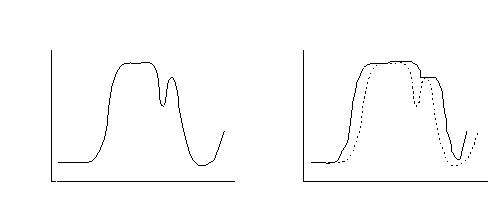
\includegraphics[width=\textwidth]{dilation}
    \caption{Dilation image intensity change}
    \label{fig:dialtion}
\end{figure}

Dilation has several use cases. It can be used to fill small spurious holes (``pepper noise"). Edge detection; performed by first taking the dilation of an image and subtracting the original image. Finally dilation forms the basis of other morphology operations in conjunction with logical operators, \textit{i.e.} region filling.


\subsubsection{Opening}

Opening is derived from the fundamental morphology operations, dilation and erosion. As such the operator requires an input image $ I $ and a structuring element $ K $. The effect of the operator is to preserve foreground regions that have a similarly shape to the structuring element, or that contain the structuring element, while eliminating all other regions of foreground pixels. 

\begin{df}Opening

Defined by erosion of $ I $ by $ K $ followed by a dilation of the product.

\begin{equation}
    I \circ K = (I \ominus K) \oplus K
\end{equation}
\end{df}

\begin{rem}
Opening can be used to remove ``salt noise" from an image. 
\end{rem}


\subsubsection{Closing}


Similar to opening, closing is defined from basic morphology operators. Closing tends to enlarge boundaries of foreground regions, but is less destructive of the original image. The operation is determined by the structuring element.


\begin{df}Closing

Defined by dilation of $ I $ by $ K $ followed by an erosion of the product.

\begin{equation}
    I \bullet K = (I \oplus K) \ominus K
\end{equation}
\end{df}

\begin{rem}
    The primary use is to fill small background holes in an image (``pepper noise"). A downside is that the dilation will distort all regions of pixels.
\end{rem}



\subsubsection{Other Operations}

\begin{df}Morphological Gradient

Is the difference between the dilation and the erosion of an image.

\begin{equation}
    I \bigtriangleup K = (I \oplus K) - (I \ominus K)
\end{equation}

\end{df}

\begin{rem}
    The resulting image will be the outline of the input image.
\end{rem}


\begin{df}Top Hat

Is the difference between the input image and the opening of the image.

\begin{equation}
    I - (I \circ K)
\end{equation}

\end{df}

\begin{df}Black Hat

Is the difference between the input image and the closing of the image.

\begin{equation}
    I - (I \bullet K)
\end{equation}

\end{df}

\subsubsection{Morphological Operations in OpenCV}


\func{cv.erode(src, kernel, iterations=1)}{Erodes an image with a specific structuring element.}

\begin{ex} Erosion

\begin{lstlisting}[language=Python]
img = cv.imread("./coins.png")
kernel = np.ones((5,5),np.uint8)
erosion = cv.erode(img, kernel, iterations=1)
\end{lstlisting}
\begin{figure}[H]
    \centering
    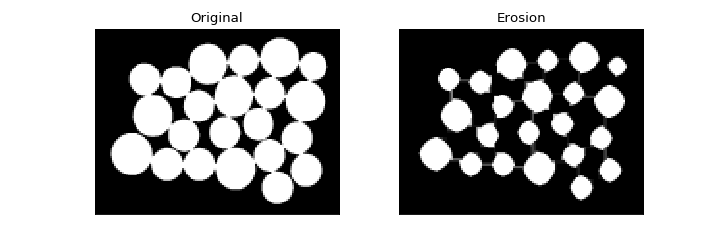
\includegraphics[width=\textwidth]{ocv_erosion}
    \caption{Erosion}
    \label{fig:ocv_ero}
\end{figure}
\end{ex}


\func{cv.dilate(src, kernel, iterations=1)}{Dilates an image by using a specific structuring element}


\begin{ex} Dilation
\begin{lstlisting}[language=Python]
kernel = np.ones((3,3),np.uint8)
dilation = cv.dilate(img, kernel, iterations=1)
\end{lstlisting}
\begin{figure}[H]
    \centering
    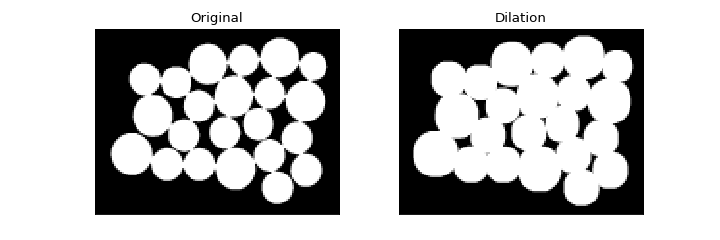
\includegraphics[width=\textwidth]{ocv_dilation}
    \caption{Dilation}
    \label{fig:ocv_dilation}
\end{figure}
\end{ex}


\func{cv.morphologyEx(src, op, kernel, iterations=1)}{Performs advanced morphological transformations}

\begin{ex} Advanced Morphology
\begin{lstlisting}[language=Python]
kernel = cv.getStructuringElement(cv.MORPH_RECT, (3, 3))
grad = cv.morphologyEx(img, cv.MORPH_GRADIENT, kernel)
\end{lstlisting}
\begin{figure}[h!]
    \centering
    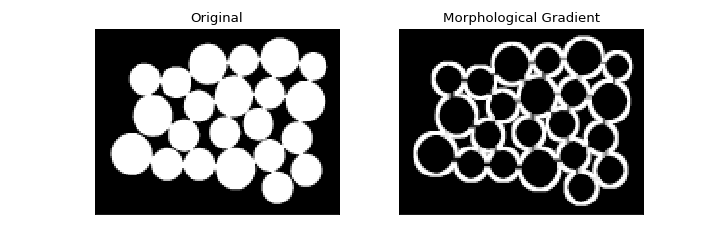
\includegraphics[width=\textwidth]{ocv_grad}
    \caption{Morphological Gradient}
    \label{fig:ocv_grad}
\end{figure}
\end{ex}

\func{cv.getStructuringElement(shape, ksize)}{Returns a structuring element of the specified size and shape for morphological operation}


\begin{table}[h!]
    \centering
    \def\arraystretch{1.1}%
    \begin{tabular}{ p{5cm} p{7cm} } 
	\hline
	Enumerator & Description \\
	\hline
	\textbf{\footnotesize{MORPH\_RECT}} & Rectangular shaped structuring element \\

	\textbf{\footnotesize{MORPH\_CROSS}} & Cross-shaped structuring element \\

	\textbf{\footnotesize{MORPH\_ELIPSE}} & An elliptic structuring element inscribed into a rectangle \\
	\hline
    \end{tabular}
    \caption{Structuring Elements}
    \label{table:col_struct_el}
\end{table}

The morphological operations are available as enumerators, and can be passed to \lstinline{morphologyEx()}.


\begin{table}[H]
    \centering
    \def\arraystretch{1.1}%
    \begin{tabular}{ p{5cm} p{7cm} } 
	\hline
	Enumerator & Description \\
	\hline
	\textbf{\footnotesize{MORPH\_ERODE}} & Erosion \\
	\textbf{\footnotesize{MORPH\_DILATE}} & Dilation \\
	\textbf{\footnotesize{MORPH\_OPEN}} & opening operation \\
	\textbf{\footnotesize{MORPH\_CLOSE}} & closing operation \\
	\textbf{\footnotesize{MORPH\_GRADIENT}} & morphological gradient \\
	\textbf{\footnotesize{MORPH\_TOPHAT}} & ``top hat" \\
	\textbf{\footnotesize{MORPH\_BLACKHAT}} & ``black hat" \\
	\textbf{\footnotesize{MORPH\_HITMISS}} & ``Hit or miss" \\
	\hline
    \end{tabular}
    \caption{Morphological Operations}
\end{table}


\break


\subsection{Image Gradients}

One of the most important uses of convolution is the computation of derivatives in an image. Image derivatives are important for detecting edges. For instance it is easy to determine an edge due to the sudden change in pixel intensity; a convenient way of expressing this change is with derivatives. 


\subsubsection{Sobel Operator}

The Sobel operator performs a 2D spatial gradient measurement on an image. It emphasises regions that correspond to edges. The operator works using a pair of kernels $ G_x \text{and } G_y $. The kernels are designed to respond maximally to edges running vertically and horizontally. Combining the products of the convolution results in the absolute magnitude.\\

\noindent The Sobel operator is given by:
\begin{equation}
    G = \sqrt{G_x^2 + G_y^2}
\end{equation}

\noindent Where:

\begin{gather*}
    G_x = \begin{bmatrix}
	-1 & 0 & +1 \\
	-2 & 0 & +2 \\
	-1 & 0 & +1 \\
    \end{bmatrix} * I \\ \\
    G_y = \begin{bmatrix}
	-1 & -2 & -1 \\
	 0 &  0 &  0 \\
	+1 & +2 & +1 \\
    \end{bmatrix} * I
\end{gather*}

\noindent The Sobel operation is performed with the \lstinline{Sobel} function.\\

\func{cv.Sobel(src, ddepth, dx, dy, ksize=3, scale=1, delta=0)}{Calculates the first, second, third or mixed image derivative using an extended Sobel operator. There is also $ \text{kszie}=-1 $ which corresponds to a $ 3 \times 3 $ Scharr filter.}

\begin{ex} Sobel Filtering
\begin{lstlisting}[language=Python]
img = cv.imread("./images/sudoku.png")
res_x = cv.Sobel(img, cv.CV_64F, 1, 0, ksize=5)
res_y = cv.Sobel(img, cv.CV_64F, 0, 1, ksize=5)
\end{lstlisting}
\begin{figure}[H]
    \centering
    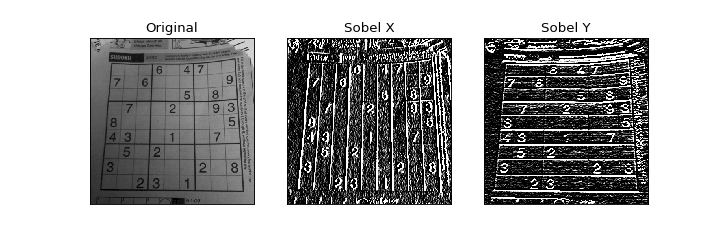
\includegraphics[width=\textwidth]{ocv_sobel}
    \caption{Sobel Filtering}
    \label{fig:ocv_sobel}
\end{figure}
\end{ex}

\begin{nb}
    By setting the Kernel size to -1 the Scharr Kernels can be applied instead of the Sobel Kernels. Scharr filtering often produces better results than Sobel filtering for smaller sized kernels. Alternatively the \lstinline{Scharr} function can be used.
\end{nb}


\subsubsection{Laplace Operator}

The Laplace Operator, denoted as $ \Delta \cdot$, is defined in terms of second derivatives. The formal mathematical definition is: 

\begin{equation}
    \Delta f = \sum_{i = 1}^{n} \frac{\partial^2 f}{\partial x_i^2}
\end{equation}

\noindent In terms of images the Laplace operator takes the second derivative  with respect to the $ x \text{ and } y $ axis.

\begin{equation}
    \Delta I = \frac{\partial^2 I}{\partial x^2} + \frac{\partial^2 I}{\partial y^2}
\end{equation}

The Laplace operator can be used as an edge detector, for instance the first derivative of an image grows rapidly when there is a change from low to high intensity, i.e. at an edge, and then decreases at a discontinuity. This implies an edge occurs at a local maxima. 


\begin{figure}[H]
    \centering
    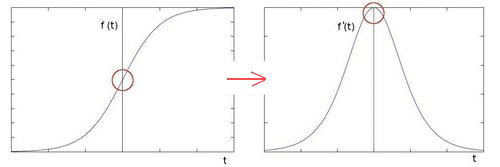
\includegraphics[width=\textwidth]{laplace_first_derv}
    \caption{First Derivative}
    \label{fig:lap_fd}
\end{figure}

Hence the second derivative of an image implies that edges occur at values around 0, i.e. the point of the local maxima.

\begin{figure}[h!]
    \centering
    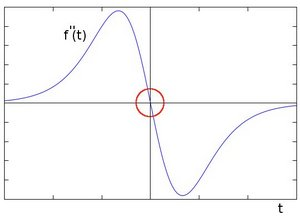
\includegraphics[width=0.5\textwidth]{laplace_sec_derv}
    \caption{Second Derivative}
    \label{fig:lap_sd}
\end{figure}

\func{cv.Laplace(src, ddepth, ksize=1, scale=1, delta=0)}{Calculates the Laplacian of an image.}

\begin{ex} Laplace Operator
\begin{lstlisting}[language=Python]
res_lap = cv.Laplacian(img, cv.CV_64F)
\end{lstlisting}
\begin{figure}[H]
    \centering
    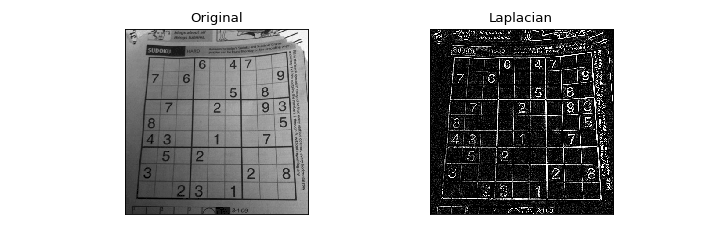
\includegraphics[width=\textwidth]{ocv_laplace}
    \caption{Laplace Operator}
    \label{fig:ocv_lap}
\end{figure}
\end{ex}

\begin{rem}
The OpenCV implementation of the Laplace Operator uses the Sobel Operator in its computation.
\end{rem}


\break


\subsection{Canny Edge Detection}

Canny edge detection uses a more sophisticated multi-staged techniques to detect edges. The function takes a grey scale image as input and produces an image showing the positions of intensity change. The operator is based on a set of particular criteria, there are other detectors that also claim to be optimal with slightly different criteria.

\subsubsection{Theory}

Canny Edge Detection begins by reducing the noise in an image with a $ 5 \times 5 $ Gaussian filter. The smoothed image is then filtered with a Sobel Kernel in both the horizontal and vertical directions. The first derivatives $ G_x \text{ and } G_y $ are then used to find the gradient and the direction of each pixel.\\

\noindent The gradient is given by: 
\begin{equation*}
    G = \sqrt{G_x^2 + G_y^2}
\end{equation*}

\noindent The direction or angle is given by:
\begin{equation}
    \theta = \tan^{-1}\bigg(\frac{G_y}{G_x}\bigg)
\end{equation}

\begin{nb}
Gradient direction is always perpendicular to edges, angles within a given range are rounded to one of four angles representing vertical, horizontal or diagonal directions.
\end{nb}

After each pixel's gradient and direction is established, the pixel is tested within its local neighbourhood to established whether it is a local maxima or not. If a pixel is not the local maxima it is set to 0, otherwise it is considered for the next stage. \\

Finally a minimum and maximum threshold, $ T_{min} \text{ and } T_{max} $ are used to determine which pixels are actually edges. Pixels with values above $ T_{max} $ are considered sure edges. Pixels between $ T_{max} \text{ and } T_{min} $ but connected to a `sure edge' are considered edges. Otherwise the pixel is discarded.

\begin{figure}[H]
    \centering
    \includegraphics[width=0.5\textwidth]{canny}
    \caption{Canny Edge Detection}
    \label{fig:canny}
\end{figure}

For instance in the above figure, Point C is connected to a sure edge (A) and so is considered as part of the final result. Point B is between the valid threshold, but not connected to a sure edge and so is discarded. The final stage is useful for removing small lines and noise which is often not considered as an edge.


\subsubsection{Canny Edge Detection in OpenCV}

\func{cv.Canny(img, minVal, maxVal, apertureSize=3, L2gradient=False)}{
Finds edges in an image using the Canny algorithm. The apertureSize is the size of the Sobel Kernel
}

\begin{ex} Canny Edge Detection
\begin{lstlisting}[language=Python]
img = cv.imread("./images/grasshopper.png", 0)
canny = cv.Canny(img, 80, 180)

# plotting
plt.figure(num=None,figsize=(9,3), dpi=80, facecolor='w',edgecolor='k')

plt.subplot(1, 2, 1)
plt.xticks([]), plt.yticks([]), 
plt.title("Original")
plt.imshow(img, cmap="gray") 

plt.subplot(1, 2, 2)
plt.xticks([]), plt.yticks([]), 
plt.title("Canny")
plt.imshow(canny, cmap="gray")

plt.show()
\end{lstlisting}
\begin{figure}[h!]
    \centering
    \includegraphics[width=\textwidth]{ocv_canny}
    \caption{Canny Edge Detection Example}
    \label{fig:ocv_canny}
\end{figure}
\end{ex}



\break

\subsection{Hough Transforms}

\subsubsection{Hough Line Transform Theory}

In the Cartesian coordinate system a line is expressed using two parameters: $ (m , c) $ giving the result: $ y = mx + c $. In Polar coordinates the same result can be expressed with parameters $ (\theta, \rho) $ as:

\begin{equation}
    y = \bigg(-\frac{\cos\theta}{\sin\theta}\bigg)x + \bigg(\frac{\rho}{\sin\theta}\bigg)
\end{equation}

\noindent Rearranging gives:
\begin{equation*}
\rho = x \cos\theta + y\sin\theta 
\end{equation*}

\noindent Hence the $ \theta, \rho $ plane can represent the set of lines that pass through a point $ (x, y) $ as shown in the following plot of the curve $ \rho = 8\cos\theta + 6\sin\theta $

\begin{figure}[H]
    \centering
    \includegraphics[width=0.5\textwidth]{hough_line}
    \caption{Set of lines that pass through $ x=8, y=6 $}
    \label{fig:hough_line}
\end{figure}

\noindent Now consider the points: $ (8,6), (4,9), (12, 3) $; drawing the curves for each in the $ \theta, \rho $ plane gives:

\begin{figure}[h!]
    \centering
    \includegraphics[width=0.5\textwidth]{hough_line_mult}
    \caption{Set of lines for points $ (8,6), (4,9), (12, 3) $}
    \label{fig:hough_line_mult}
\end{figure}

\noindent Intersecting curves imply that all the points belong to the same line.\\

The Hough Line Transform keeps track of the intersections between the curves of every point in an image. If the number of intersections is above some threshold, then it declares it as a line with the parameters $ (\theta, \rho_{\theta}) $ of the intersection point.

\subsubsection{Hough Line transform in OpenCV}

OpenCV implements two kinds of Hough line transforms: Standard and Probabilistic.

\begin{nb}
The Probabilistic implementation only considers a random subset of points in order to detect lines.
\end{nb}

\func{cv.HoughLines(img, rho, theta, threshold)}{Finds lines in a binary image using the Standard Hough transform.}\\

\func{cv.HoughLinesP(img, rho, theta, threshold)}{Finds line segments in a binary image using the Probabilistic Hough transform.}

\begin{ex} Hough Line Transform
\begin{lstlisting}[language=Python]
img = cv.imread("./images/sudoku.png")
img_2 = img.copy()
gray = cv.cvtColor(img, cv.COLOR_BGR2GRAY)
edges = cv.Canny(gray, 50, 150)

# Standard
hough_pts_std = cv.HoughLines(edges, 1, np.pi/100, 200)

for line in hough_pts_std:
    rho,theta = line[0]
    a = np.cos(theta)
    b = np.sin(theta)
    x0 = a*rho
    y0 = b*rho
    x1 = int(x0 + 1000*(-b))
    y1 = int(y0 + 1000*(a))
    x2 = int(x0 - 1000*(-b))
    y2 = int(y0 - 1000*(a))
    cv.line(img,(x1,y1),(x2,y2),(0,0,255),2)

# Probabilistic
hough_pts_prob = cv.HoughLinesP(edges, 1, np.pi/100, 100, minLineLength=100, maxLineGap=10)

for line in hough_pts_prob:
    x1,y1,x2,y2 = line[0]
    cv.line(img_2,(x1,y1),(x2,y2),(0,255,0),2)
\end{lstlisting}
\begin{figure}[H]
    \centering
    \includegraphics[width=\textwidth]{ocv_hlt}
    \caption{Hough Line Transform}
    \label{fig:ocv_hlt}
\end{figure}
\end{ex}

\subsubsection{Hough Circle Transform Theory}

The Hough Circle Transform works similarly to the Hough Line Transform. However three parameters are needed to define a circle: 

\begin{equation*}
 (x_{center}, y_{center}, r) 
\end{equation*}

\noindent The increased dimensionality of the problem, \textit{i.e.} the consideration of the radius $ r $, means the problem is computationally more intense; OpenCV implements a method known as the Hough gradient method to determine these values.

The Hough gradient method works by first passing an image through an edge detector, in this case the \lstinline{cv.Canny()} function. For every non-zero pixel in the edge image, the local gradient is computed via the first-order Sobel derivatives. Using the gradient, a set of lines is determined constrained by the specified minimum and maximum radial distance, every point that lies on one of these lines is added to an accumulator. Using the non-zero pixels in the edge image, the candidate centres are determined and sorted in descending order based on their accumulator values. Therefore the centres with the most supporting pixels appear first. Using the pixels in the accumulator list described earlier, the pixels are sorted based on their distance from the centre, a radius is selected which is closest to the specified maximum radius. A centre is kept if it has sufficient support from the non-zero pixels in the edge image and if it is a sufficient distance from any previously selected circle.

\subsubsection{Hough Circle Transform in OpenCV}

\func{cv.HoughCircles(img, method, dp, minDist, param1=100, param2=100, minRadius=0, maxRadius=0)}{
    Finds circles in a grayscale image using the Hough Transform. Returns an output vector of found circles.\\ 
    \begin{tabular}{ p{2cm} p{10cm} }
	\indent\lstinline{dp} & is the accumulator resolution, i.e. a value of 2 means the accumulator has half the resolution as the input image\\
	\indent\lstinline{minDist} & is the minimum distance between circles\\ 
	\indent\lstinline{param1} & is the higher threshold passed to the Canny edge detector\\ 
	\indent\lstinline{param2} & is the accumulator threshold, a lower value may detect more false circles.
    \end{tabular}
}


\begin{ex} Hough Circle Transform
\begin{lstlisting}[language=Python]
# load image
img = cv.imread("./images/coins_2.png")

# process image
img = cv.medianBlur(img, 7)
img_gr = cv.cvtColor(img, cv.COLOR_BGR2GRAY)
img_edg = cv.Canny(img_gr, 100, 200)

# apply hough circle transform
circles = cv.HoughCircles(img_gr, cv.HOUGH_GRADIENT, 1, 
		minDist=60, param1=200, param2=40, 
		minRadius=30, maxRadius=200)

circles = np.uint16(np.around(circles))

for cir in circles[0,:]:
    center = (cir[0], cir[1])
    rad = cir[2]
    # draw the outer circle
    cv.circle(img, center, rad, (0,255,0), 20)
    # draw marker at center
    cv.circle(img, center, 20, (0,0,255), -1)
\end{lstlisting}

\begin{figure}[H]
    \centering
    \includegraphics[width=\textwidth]{ocv_hough_circ}
    \caption{Hough Circle Transform with Coins}
    \label{fig:ocv_hct}
\end{figure}
\end{ex}


\break 


\section{OpenCV: Image Processing - Segmentation}

\subsection{Image Contours}




\end{document}
